%%%%%%%%%%%%%%%%%%%%%%%%%%%%%%%%%%%%%%%%%%%%%%%%%%%%
% Document type, global settings, and packages
%%%%%%%%%%%%%%%%%%%%%%%%%%%%%%%%%%%%%%%%%%%%%%%%%%%%

\documentclass[12pt]{report}   %12 point font for Times New Roman
\usepackage{graphicx}  %for images and plots
\usepackage[letterpaper, left=1.5in, right=1in, top=1in, bottom=1in]{geometry}
\usepackage{setspace}  %use this package to set linespacing as desired
\usepackage{times}  %set Times New Roman as the font
\usepackage[explicit]{titlesec}  %title control and formatting
\usepackage[titles]{tocloft}  %table of contents control and formatting
\usepackage[backend=bibtex, sorting=none, bibstyle=ieee]{biblatex}  %reference manager
\usepackage[bookmarks=true, hidelinks]{hyperref}
\usepackage[page]{appendix}  %for appendices
\usepackage{rotating}  %for rotated, landscape images
\usepackage[normalem]{ulem}  %for italicized text
\usepackage{amsmath}
\usepackage{amssymb}
\usepackage{subcaption}
\usepackage{multirow}
\usepackage{dcolumn}
\usepackage{url}


\newcolumntype{d}[1]{D{.}{.}{#1} }
%the argument for d specifies the maximum number of decimal places


%%%%%%%%%%%%%%%%%%%%%%%%%%%%%%%%%%%
% Bibliography
%%%%%%%%%%%%%%%%%%%%%%%%%%%%%%%%%%%

%Add your bibliography file here
\bibliography{references}

% prevent certain fields in references from printing in bibliography
\AtEveryBibitem{\clearfield{issn}}
\AtEveryBibitem{\clearlist{issn}}

\AtEveryBibitem{\clearfield{language}}
\AtEveryBibitem{\clearlist{language}}

\AtEveryBibitem{\clearfield{doi}}
\AtEveryBibitem{\clearlist{doi}}

\AtEveryBibitem{\clearfield{url}}
\AtEveryBibitem{\clearlist{url}}

\AtEveryBibitem{%
  \ifentrytype{online}
    {}
    {\clearfield{urlyear}\clearfield{urlmonth}\clearfield{urlday}}}

%%%%%%%%%%%%%%%%%%%%%%
% Start of Document
%%%%%%%%%%%%%%%%%%%%%%

\begin{document}
\doublespacing  %set line spacing

%%%%%%%%%%%%%%%%%%%%%%%%%%%%%%%%%%%%%
% Title Page
%%%%%%%%%%%%%%%%%%%%%%%%%%%%%%%%%%%%%

%% Define your thesis title, your name, your school, and your month and year of graduation here

\newcommand{\thesisTitle}{Real time detection of traffic signs on mobile device}
\newcommand{\yourName}{Nicolas \textsc{Six}}
\newcommand{\yourSchool}{Computer Science}
\newcommand{\yourMonth}{December}
\newcommand{\yourYear}{2019}

%%%%%%%%%%%%%%%%%%%%%%%%%%%%%%%%%%%%%%%%%%%%%%%%%%%%%%%%%
% Do not edit these lines unless you wish to customize
% the template
%%%%%%%%%%%%%%%%%%%%%%%%%%%%%%%%%%%%%%%%%%%%%%%%%%%%%%%%%



\begin{titlepage}
\begin{center}

\begin{singlespacing}

\textbf{\MakeUppercase{\thesisTitle}}\\
\vspace{10\baselineskip}
A Dissertation\\
Presented to\\
The Academic Faculty\\
\vspace{3\baselineskip}
By\\
\vspace{3\baselineskip}
\yourName\\
\vspace{3\baselineskip}
In Partial Fulfillment\\
of the Requirements for the Degree\\
Master of Computer Science in the\\
School of \yourSchool\\
\vspace{3\baselineskip}
Georgia Institute of Technology\\
\vspace{\baselineskip}
\yourMonth{} \yourYear{}
\vfill
Copyright \copyright{} \yourName{} \yourYear{}

\end{singlespacing}

\end{center}
\end{titlepage}



\currentpdfbookmark{Title Page}{titlePage}  %add PDF bookmark for this page

%%%%%%%%%%%%%%%%%%%%%%%%%%%%%%%%%%%%%
% Approval Page
%%%%%%%%%%%%%%%%%%%%%%%%%%%%%%%%%%%%%

%% Define your committee members. If you have less than 6, simple delete/comment the unused lines

\newcommand{\committeeMemberOne}{Dr. Kira, Advisor}
\newcommand{\committeeMemberOneDepartment}{School of Interactive Computing}
\newcommand{\committeeMemberOneAffiliation}{Georgia Institute of Technology}

\newcommand{\committeeMemberTwo}{Dr. Tsai, Co-Advisor}
\newcommand{\committeeMemberTwoDepartment}{School of Civil and Environmental Engineering}
\newcommand{\committeeMemberTwoAffiliation}{Georgia Institute of Technology}

\newcommand{\committeeMemberThree}{Dr. Wang}
\newcommand{\committeeMemberThreeDepartment}{Center for Spatial Planning Analytics and Visualization}
\newcommand{\committeeMemberThreeAffiliation}{Georgia Institute of Technology}

% \newcommand{\committeeMemberFour}{Dr. Four}
% \newcommand{\committeeMemberFourDepartment}{School of Computer Science}
% \newcommand{\committeeMemberFourAffiliation}{Georgia Institute of Technology}

% \newcommand{\committeeMemberFive}{Dr. Five}
% \newcommand{\committeeMemberFiveDepartment}{School of Public Policy}
% \newcommand{\committeeMemberFiveAffiliation}{Georgia Institute of Technology}

% \newcommand{\committeeMemberSix}{Dr. Six}
% \newcommand{\committeeMemberSixDepartment}{School of Nuclear Engineering}
% \newcommand{\committeeMemberSixAffiliation}{Georgia Institute of Technology}

\newcommand{\approvalDay}{$3^{rd}$}
\newcommand{\approvalMonth}{December}
\newcommand{\approvalYear}{2019}

%%%%%%%%%%%%%%%%%%%%%%%%%%%%%%%%%%%%%%%%%%%%%%%%%%%%%%%%%
% Do not edit these lines unless you wish to customize
% the template
%%%%%%%%%%%%%%%%%%%%%%%%%%%%%%%%%%%%%%%%%%%%%%%%%%%%%%%%%


\begin{titlepage}
\begin{singlespacing}
\begin{center}

\textbf{\MakeUppercase{\thesisTitle}}\\
\vspace{10\baselineskip}

\end{center}
\vfill

%Define minipages, depending on how many authors there are
\ifdefined\committeeMemberFour

Approved by:
\vspace{2\baselineskip}		%adjust the number in front of "\baselineskip" for alignment

\begin{minipage}[b]{0.4\textwidth}
	
	\committeeMemberOne\\
	\committeeMemberOneDepartment\\
	\textit{\committeeMemberOneAffiliation}\\
	
	\committeeMemberTwo\\
	\committeeMemberTwoDepartment\\
	\textit{\committeeMemberTwoAffiliation}\\
	
	\committeeMemberThree\\
	\committeeMemberThreeDepartment\\
	\textit{\committeeMemberThreeAffiliation}\\
	
	\vspace{2\baselineskip}		%adjust the number in front of "\baselineskip" for alignment
	
\end{minipage}
\hspace{0.1\textwidth}
\begin{minipage}[b]{0.4\textwidth}
	
% 	\committeeMemberFour\\
% 	\committeeMemberFourDepartment\\
% 	\textit{\committeeMemberFourAffiliation}\\
	
	\ifdefined\committeeMemberSix
	\committeeMemberFive\\
	\committeeMemberFiveDepartment\\
	\textit{\committeeMemberFiveAffiliation}\\
	
	\committeeMemberSix\\
	\committeeMemberSixDepartment\\
	\textit{\committeeMemberSixAffiliation}\\
	
	Date Approved: \approvalMonth{} \approvalDay, \approvalYear
	\vspace{1\baselineskip}		%adjust the number in front of "\baselineskip" for alignment
	
	\else
	
	\committeeMemberFive\\
	\committeeMemberFiveDepartment\\
	\textit{\committeeMemberFiveAffiliation}\\
		
	Date Approved: \approvalMonth{} \approvalDay, \approvalYear
	\vspace{5\baselineskip}		%adjust the number in front of "\baselineskip" for alignment
	
	\fi
	
\end{minipage}

\else

\hspace{0.6\textwidth}
\begin{minipage}[b]{0.4\textwidth}
	
	Approved by:
	\vspace{2\baselineskip}		%adjust the number in front of "\baselineskip" for alignment
	
	\committeeMemberOne\\
	\committeeMemberOneDepartment\\
	\textit{\committeeMemberOneAffiliation}\\
	
	\committeeMemberTwo\\
	\committeeMemberTwoDepartment\\
	\textit{\committeeMemberTwoAffiliation}\\
	
	\committeeMemberThree\\
	\committeeMemberThreeDepartment\\
	\textit{\committeeMemberThreeAffiliation}\\
	
	\vspace{2\baselineskip}		%adjust the number in front of "\baselineskip" for alignment
	
	Date Approved: \approvalMonth{} \approvalDay, \approvalYear
	\vspace{\baselineskip}		%adjust the number in front of "\baselineskip" for alignment
	
\end{minipage}

\fi





\end{singlespacing}
\end{titlepage}


%%%%%%%%%%%%%%%%%%%%%%%%%%%%%%%%%%%%%
% Epigraph
%%%%%%%%%%%%%%%%%%%%%%%%%%%%%%%%%%%%%

% Define your quote and author for the epigraph here

\newcommand{\yourQuote}{
\includegraphics[width=.5\linewidth]{figures/machine_learning.png}}
\newcommand{\yourAuthor}{Randall Munroe}

%%%%%%%%%%%%%%%%%%%%%%%%%%%%%%%%%%%%%%%%%%%%%%%%%%%%%%%%%
% Do not edit these lines unless you wish to customize
% the template
%%%%%%%%%%%%%%%%%%%%%%%%%%%%%%%%%%%%%%%%%%%%%%%%%%%%%%%%%

\begin{titlepage}
\begin{center}

\vspace*{\fill}
\yourQuote\\
\textit{\yourAuthor}
\vspace*{\fill}

\end{center}
\end{titlepage}



%%%%%%%%%%%%%%%%%%%%%%%%%%%%%%%%%%%%%
% Dedication
%%%%%%%%%%%%%%%%%%%%%%%%%%%%%%%%%%%%%

% Define your dedication statement here

\newcommand{\yourDedication}{To anyone that will take the time to read it,}

%%%%%%%%%%%%%%%%%%%%%%%%%%%%%%%%%%%%%%%%%%%%%%%%%%%%%%%%%
% Do not edit these lines unless you wish to customize
% the template
%%%%%%%%%%%%%%%%%%%%%%%%%%%%%%%%%%%%%%%%%%%%%%%%%%%%%%%%%

\begin{titlepage}
\begin{center}

\vspace*{\fill}
\yourDedication\\
\vspace*{\fill}

\end{center}
\end{titlepage}


%%%%%%%%%%%%%%%%%%%%%%%%%%%%%%%%%%%%%
% Acknowledgments
%%%%%%%%%%%%%%%%%%%%%%%%%%%%%%%%%%%%%

\pagenumbering{roman}
\addcontentsline{toc}{chapter}{Acknowledgments}
\setcounter{page}{5} % set the page number appropriately based on the number of intro pages
\clearpage
\begin{centering}
\textbf{\textsc{Acknowledgments}}\\
\vspace{\baselineskip}
\end{centering}

%Insert your dedication text here

%Cibi ZongYu data collection
%Sai Gogineni annotation

This work would not have been possible without the support and continuous advice of Dr. Tsai. The structure and organization of his team made this work a reality, by providing high quality data and the needed hardware to set up the experiments. A special thanks to Dr. Kira, who made this thesis possible, and gave me some precious advice. My only regret is not to have asked more question to him.

We also want to thank particularly Cibi Pranav, Ryan Salameh and Zhongyu Yang for the data they collected during their various trip around Georgia and neighboring states. As well as a great thanks to Sai Gogineni, who annotated by himself all $652,321$ frames collected, creating the dataset we used during this study.

Thanks to Cindy for proofreading most of this work and for her continuous support.


\clearpage
%\pagenumbering{gobble}  %remove page number on summary page


%\addtocontents{toc}{\cftpagenumbersoff{chapter}} 

%\currentpdfbookmark{Acknowledgments}{acknowledgments}
%\addtocontents{toc}{\cftpagenumberson{chapter}} 

%%%%%%%%%%%%%%%%%%%%%%%%%%%%%%%%%%%%%
% Table of Contents
%%%%%%%%%%%%%%%%%%%%%%%%%%%%%%%%%%%%%

% Format for Table of Contents
\renewcommand{\cftchapdotsep}{\cftdotsep}  %add dot separators
\renewcommand{\cftchapfont}{\bfseries}  %set title font weight
\renewcommand{\cftchappagefont}{}  %set page number font weight
\renewcommand{\cftchappresnum}{Chapter }
\renewcommand{\cftchapaftersnum}{:}
\renewcommand{\cftchapnumwidth}{5em}
\renewcommand{\cftchapafterpnum}{\vskip\baselineskip} %set correct spacing for entries in single space environment
\renewcommand{\cftsecafterpnum}{\vskip\baselineskip}  %set correct spacing for entries in single space environment
\renewcommand{\cftsubsecafterpnum}{\vskip\baselineskip} %set correct spacing for entries in single space environment
\renewcommand{\cftsubsubsecafterpnum}{\vskip\baselineskip} %set correct spacing for entries in single space environment

%format title font size and position (this also applys to list of figures and list of tables)
\titleformat{\chapter}[display]
{\normalfont\bfseries\filcenter}{\chaptertitlename\ \thechapter}{0pt}{\MakeUppercase{#1}}

\renewcommand\contentsname{Table of Contents}

\begin{singlespace}
\tableofcontents
\end{singlespace}

\currentpdfbookmark{Table of Contents}{TOC}

\clearpage

%%%%%%%%%%%%%%%%%%%%%%%%%%%%%%%%%%%%%
% List of figures and tables
%%%%%%%%%%%%%%%%%%%%%%%%%%%%%%%%%%%%%

\addcontentsline{toc}{chapter}{List of Tables}
\begin{singlespace}
	\setlength\cftbeforetabskip{\baselineskip}  %manually set spacing between entries
	\listoftables
\end{singlespace}

\clearpage

\addcontentsline{toc}{chapter}{List of Figures}
\begin{singlespace}
\setlength\cftbeforefigskip{\baselineskip}  %manually set spacing between entries
\listoffigures
\end{singlespace}

\clearpage

%%%%%%%%%%%%%%%%%%%%%%%%%%%%%%%%%%%%%%%%%%%%%%%%%%%%%%%%%%%%%%%%%
% This is the Summary (abstract should be separate document)
%%%%%%%%%%%%%%%%%%%%%%%%%%%%%%%%%%%%%%%%%%%%%%%%%%%%%%%%%%%%%%%%%

\clearpage
\begin{centering}
\textbf{SUMMARY}\\
\vspace{\baselineskip}
\end{centering}

In this work we propose a new approach to the object detection problem using Deep Neural Network, in the context of traffic sign detection. Our approach simplifies the detection head complexity by making the requirement for localization lower and taking advantage of our particular task to make the feature extraction model smaller. This strategy allows to create a model running at $88$ frames per second on a four years old smartphone, a Samsung S6 (SM-G920T), while maintaining a mAP@50 at $55\%$ and mAP@25 at $68\%$.

To get these results, we created a way to generate data for training based on random geometrical shapes that allows to initialize the weights of our model before training on real data.

To the best of our knowledge this model provides the best accuracy over speed ratio for the detection of traffic signs on mobile device at the moment.

%\pagenumbering{gobble}  %remove page number on summary page

%%%%%%%%%%%%%%%%%%%%%%%%%%%%
%
% Chapters
%
%%%%%%%%%%%%%%%%%%%%%%%%%%%%

%%%%%%%%%%%%%%%%%%%%%%
% formatting
%%%%%%%%%%%%%%%%%%%%%%

% resume page numbering for rest of document
\clearpage
\pagenumbering{arabic}
\setcounter{page}{1} % set the page number appropriately

% Adjust chapter title formatting
\titleformat{\chapter}[display]
{\normalfont\bfseries\filcenter}{\MakeUppercase\chaptertitlename\ \thechapter}{0pt}{\MakeUppercase{#1}}  %spacing between titles
\titlespacing*{\chapter}
  {0pt}{0pt}{30pt}	%controls vertical margins on title
  
% Adjust section title formatting
\titleformat{\section}{\normalfont\bfseries}{\thesection}{1em}{#1}

% Adjust subsection title formatting
\titleformat{\subsection}{\normalfont}{\uline{\thesubsection}}{0em}{\uline{\hspace{1em}#1}}

% Adjust subsubsection title formatting
\titleformat{\subsubsection}{\normalfont\itshape}{\thesubsection}{1em}{#1}

%%%%%%%%%%%%%%%%
% Chapter 1
%%%%%%%%%%%%%%%%

\chapter{Introduction and Background}
\label{litreview}

\section{Introduction}
\paragraph{}
The quest of achieving autonomous driving is not new, much research has been focused on this area since the early 1990s. Sign detection is part of that quest and so gets a fair amount of attention by the research community and industry alike. The applications range from experimental self-driving vehicles to common driver assistance hardware. The constant progress of computer vision techniques and the progress made on hardware constantly reshape the boundary of possibility to run real time detection on low end embedded hardware.

In this Chapter we will review the different methods explored by the research community to try to solve traffic sign detection problem. We will first focus on the pre-deep learning area algorithms, which will be noted as classical algorithms in this document, and try to exhibit the different methods they tried and how they already incorporated machine learning to improve their results. We will then focus on how deep learning changed image processing and introduce some state of the art object detection models. We also explore new possibilities offered by approaches like architecture search and the current focus on mobile devices.

\section{Traffic sign detection}
\paragraph{}
Traffic sign detection has a long history that started as soon as RGB digital camera became available. In 1993, \cite{janssen1993hybrid, besserer1993shape} were already trying to solve this problem. The approach proposed by \cite{janssen1993hybrid} is based on per color pixel classification to segment the potential sign on the image followed by a pictogram classifier, while the approach proposed by \cite{besserer1993shape} reposed on grayscale image to lower the computation requirement and used multi-scale grayscale segmentation to extract shapes and classify them.

Some autonomous prototypes were also developed in the year 1994 \cite{ulmer1994vita}. The vehicle presented in \cite{ulmer1994vita} needed an additional $1400W$ power supply to run the embedded equipment while the document states "the complexity of this [traffic sign] recognition task".

With the progress of computer vision and computational power of computers, more complex approachs have now been explored. \cite{de1997road} proposes a method based on color threshold and edge detection to perform this task and introduces a fully connected neural network to perform the classification. Another method of threshold using both HSV and YUV color space to better take into account the different illuminations was proposed in \cite{shadeed2003road}, while \cite{bahlmann2005system} proposed a new approach using Haar wavelet transform of the image and performing detection by extracting features of this transformation based on an Ada-boost trained classifier.

As more computational power became available, it became clear that computer vision algorithms needed machine learning to fine tune their algorithms, and as such data started to appear as a cornerstone of this task. In addition, the rapid development of the world wide web provided an easy way to share data across the scientific community, making the process of comparing results easier. Data set such as GTSDB \cite{gtsdb} quickly appeared to fill that gap, proposing a set of one thousand images from German roads, properly annotated, to the community. Other data set quickly followed such as \cite{mathias2013traffic} in Belgium or \cite{larssonSCIA2011} in Sweden.

\paragraph{}
The methods presented above manage to get good accuracy on detection with a relatively low computation budget by today's standards. However, the results often lack the repeatability needed for real word application and are specific to the setup of the authors.

\section{Deep learning}
\paragraph{}
Since the demonstration done with AlexNet \cite{alexnet} on the ImageNet \cite{deng2009imagenet}, deep learning have received much attention from the research community and the industry. This interest lead to major breakthroughs in computer vision tasks, starting from image classification and propagating to object detection, image segmentation or image captioning. This revolution in the computer vision field was lead by the use of powerful GPU allowing running complex models.
\subsection{Image Classification}
\paragraph{}
AlexNet \cite{alexnet} opened the gate to a large amount of innovation. Resnet \cite{szegedy2017inception} showed that residual connection allowed the gradient to propagate further in the network.

Other architecture such as MobileNet \cite{sandler2018mobilenetv2, howard2019mobilenetv3} were also developed to fit particular hardware platforms or tasks. Trying to be more optimized for mobile devices by using operation that are more efficient on a sequential CPU, and not on big parallel GPU as it is usually done.

\subsection{Object detection}
\paragraph{}
Object detection was part of the second wave of deep learning. In this case, this new approach also allowed to reach accuracy never reached before. The goal here is to have a system that provides boxes around a specific set of objects when given an image. This field is dominated by two approaches that now tends to get closer and closer.

The first approach to solve this problem was to first have a region proposal network that detects objects and a classifier giving the class of the object. This approach was successfully shown in RCNN \cite{girshick2014rich}, but the process was later shown to be inefficient and was streamlined into a single module in Fast-RCNN \cite{girshick2015fast} allowing a faster detection speed and a single stage training. This process was improved even more in Faster-RCNN \cite{ren2015faster}, which makes the detection even faster by using the same feature extraction layers for region proposal and object classification, cutting the computation time required, but was still not able to reach real time object detection even on big GPU.

The second approach is very similar to Faster-RCNN in that it needs only to run on the image once and use the same feature extraction for all the predictions, but instead of doing a two steps process, here the networks predict directly the bounding boxes shape and class on the same layer. Usually these prediction layers are then placed at different depths of the network to manage different sizes. This approach was first demonstrated on YOLO \cite{yolov3}, allowing running detection real time with only a small accuracy loss over Faster-RCNN. This process was generalized with SSD \cite{liu2016ssd} that follows the same idea but with small changes that make it easier to use with different backbone networks.

One common point of the object detection methods is that they have a tendency to predict multiple boxes for the same object. To remove that problem, a post processing step is often needed. Usually this post processing is done by a non max suppression algorithm. This algorithm takes as input a threshold value between $0$ and $1$, and compares the intersection over union of each predicted boxes pair, removing one of the boxes if this value is higher than the threshold and leaving only the box with the higher confidence level. This approach allows to remove most of the duplicate detection, even if it sometimes harm the results in case of superposing objects.

Object detection is now a problem that is considered to be nearly solved by the research community, as models like Yolo and Faster-RCNN manage to achieve above human performance. However, getting this kind of results require both a very large amount of data for training as well as a very powerful GPU to run it at a reasonable frame rate.


\subsection{Architecture search} \label{architectureSearch}
\paragraph{}
Architecture search is currently a very active area in the research community. It is also a problem that is still unsolved. This area of research start from the observation that the current network architectures used globally are designed by experts to solve their current problems. However, these networks are limited to specific problems and may not be optimal to solve other problem. The idea is then to train a computer to generate architecture that can be trained and achieve better or as good as human designed ones.

The most common approach to this problem is to train a network to design another network. This is usually done with a Recurrent Neural Network (RNN) trained using Reinforcement Learning (RL) to design an architecture \cite{zoph2016neural}.

Another approach is to rely on genetic algorithm to select the evolution of the network. This technique was demonstrated in \cite{real2019regularized} and showed impressive results on the ImageNet \cite{deng2009imagenet} image classification challenge. 

The last way that is currently investigated is to make the architecture differentiable so that you can train it at the same time as the weights during gradient decent. This method was successfully used in \cite{liu2018darts} and show interesting results in term of training time as well as quality.

The above approaches are usually combined with more classical exploration approaches like NetAdapt \cite{yang2018netadapt}, which tries to further improve the global architecture to a target device. 

However, those approaches still require a fair amount of time and computing power. In addition, this research area mainly focuses on image classification so far, and being a very active topic there is no reference implementation.

\subsection{Mobile device} \label{subsec:optMobileDevice}
\paragraph{}
Nowadays the problem of object detection is largely solved. It still requires a large amount of data which are not available in every field, but given enough data you can detect objects in real time with while being more accurate than humans. However, this approach is still very heavy in computations and require large computer and GPU to run effectively. This causes trouble for many applications where you would like to process the data while collecting them, either because you need to interact with your environment or because you cannot manage the data generated by recording everything. In addition, most of the time you cannot afford to bring a powerful computer with GPU to collect your data and prefer to use more broadly available devices.

The first step in improving performance is to scale the network down, this can be done in multiple ways, as discussed in Section \ref{architectureSearch}. To improve further you have to go to hardware specific optimization. In this area, weight quantification is the most used technique. This approach consists of changing the commonly used 32 bits floating-point values to 8 bits integer values. A method leveraging SSE instruction set on an Intel CPU can provide large speed up to the run time when combined to conversion from floating-point to integer value was presented in \cite{vanhoucke2011improving}. \cite{jacob2017quantization} and \cite{gysel2016hardwareoriented} show that a similar approach can be used for mobile devices and have shown to have a large impact on prediction speed of the optimized networks.

However, optimizing the network further is not always possible. To make devices smarter, manufacturers now bundle more and more computational power in their devices. Smartphones are a good demonstrator of this trend, with newer models getting much larger and accessible parallel computation unit, sometimes even proposing additional chip to run neural networks. Following this trend Google is developing a smaller version of their TPU for mobile device under the name Coral. A similar trend is going on Internet Of Things (IoT) devices. Completing computations on site is a key factor to save space and bandwidth. Coral devices are not the only one the to target this; Nvidia released many different development board with large integrated GPU with a strong incentive on self driving cars.

\subsection{Training}
\paragraph{}
One of the biggest challenges of machine learning is overfitting. Artificial neural networks are very sensitive to this because of the high number of parameters they use. Because of that they are also very difficult to train on a reasonable time scale. These problems are well known and were subject of lot of research, leading in large improvements on that field. We are going to quickly cover some of the improvements that are used in this work.

The original inspiration for artificial neural network are the real neural networks we find in animals brains. Much of early design choices were made following this idea. A good example of that is the activation function. Activation function need to be non-linear to add expressivity to the network and prevent it from being collapsible into one linear function. Originally, $sigmoid$ function was used as they provided a good equivalent to animal brains, this function was later ruled out by $tanh$ that provided easier training by centering the output values around zero. However, this function is computationally intensive and was later replaced by ReLu, a function defined as $ReLu(x) := max(0,x)$. This function was proven to allow good training while making it easier to compute. Cropping this activation function upward has also been proven to be more effective on mobile devices \cite{sandler2018mobilenetv2, howard2019mobilenetv3}, leading to the adoption of the ReLu6 function, defined as $ReLu6 := min(6,ReLu(x))$. The research on activation function is still ongoing, the sift activation function used in \cite{howard2019mobilenetv3} has allowed to improve the results, but at a higher computational cost. In this study we chose to use the ReLu6 activation function for its efficiency.

It quickly became apparent that the distribution of the activation in the hidden layer was slowing down the training. Instead of expecting the gradient decent to fix that during training, one approach was shown to be very successful, batch normalization \cite{ioffe2015batch}. Batch normalization learns during the training to do an approximate normalization over each training batch and applies it during prediction time, making the following layers more effective.

Batch normalization has a tendency to reduce overfitting, but is far from solving this issue. On image based network, like in this work, it is easy to tweak the images slightly to add more diverse cases to the training and prevent the network from overfitting the training data. These modification are usually color shift, brightness change, or linear transformation such as rotation, translation and zoom. A more generic approach to prevent this problem is Dropout \cite{srivastava2014dropout}. This approach proposes to randomly disable connection in a neural network during the training, forcing the network to build some redundancy and preventing it from relying on only one feature. This approach has proven to be very effective in a large spectrum of cases across all fields where neural networks are used. However, the final results will always depend on the quality and quantity of real world data available.

This is only a quick review of the most used ways to improve neural network training time and accuracy, focusing on the methods we are going to use in this study.

\section{Metrics}
\subsection{Introduction}
\paragraph{}
In this work we are going to use different metrics to evaluate our results. The reader who is already familiar with the concept of IoU or mAP may decide to skip this section.

\subsection{Intersection over Union}
\paragraph{}
Intersection over Union or IoU, is the most used way to check if two objects are correctly overlapping or not. The name of this metric is self explanatory: the value of this metric is the value of the division of the area of the intersection over the area of the union, as you can see illustrated on Figure \ref{fig:iou}.

\begin{figure}
    \centering
    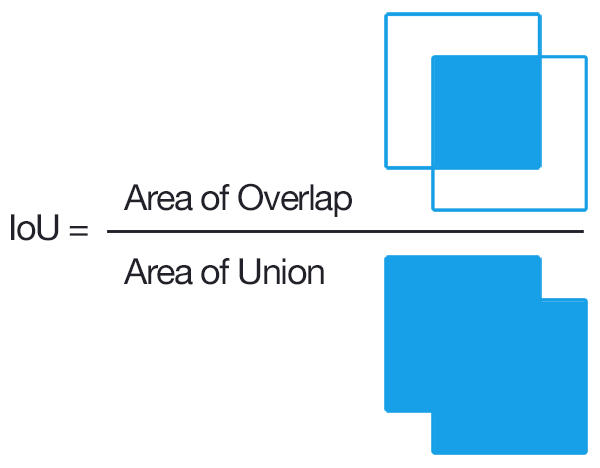
\includegraphics[width=0.3\linewidth]{figures/Intersection_over_Union_-_visual_equation.png}
    \caption{Illustration of intersection over union equation from \cite{wiki:iou}}
    \label{fig:iou}
\end{figure}{}

The value of this metric is equal to one if and only if the to area are exactly overlapping. The value decrease to zero as the overlapping become less important, taking into account the fact that one of the object may be inside the other. This makes it a great metric to compare a predicted box with a ground truth box.

\subsection{True positive, false positive and false negative}
\paragraph{}
In a object detection context, True Positive, False Positive and False Negative, often written as TP, FP and FN, are values that, in a nutshell, represent respectively the count of detection matching the ground truth, not matching the ground truth and ground truth not matched with any detection. 

First we need to define what is a match between detection and ground truth. This is usually defined by using the IoU between the two boxes, creating a match if the IoU value is above a given threshold. In this work as it is generally the case in the literature, unless explicitly stated otherwise, the threshold we use is $0.5$. So a detection match a ground truth if the IoU between them is higher than $50\%$.

With that definition set, we can come back to the previous statement. If a detection is matched with a ground truth, this detection is counted as a TP. After matching, all the remaining unmatched detection are FP and the unmatched ground truth are FN.

For the sake of simplicity we skipped here the case of multiple detection matching the same ground truth. In this case the higher IoU match is kept, so the ground truth is only matched once.

\subsection{Precision and Recall}
\paragraph{}
Using the TP, FP and FN values defined previously we can build more meaningful metrics, such as precision and recall. As illustrated by Figure \ref{fig:precisionrecall}, precision and recall answers two different questions. The first answers the question of how many of detected objects are relevant, putting the incentive on the FP as a maximum precision can only be reach if there is no FP, but without paying attention to FN. On the other hand, recall tries to answer the question of how many of the truth object were detected, but without considering FP.

\begin{figure}
    \centering
    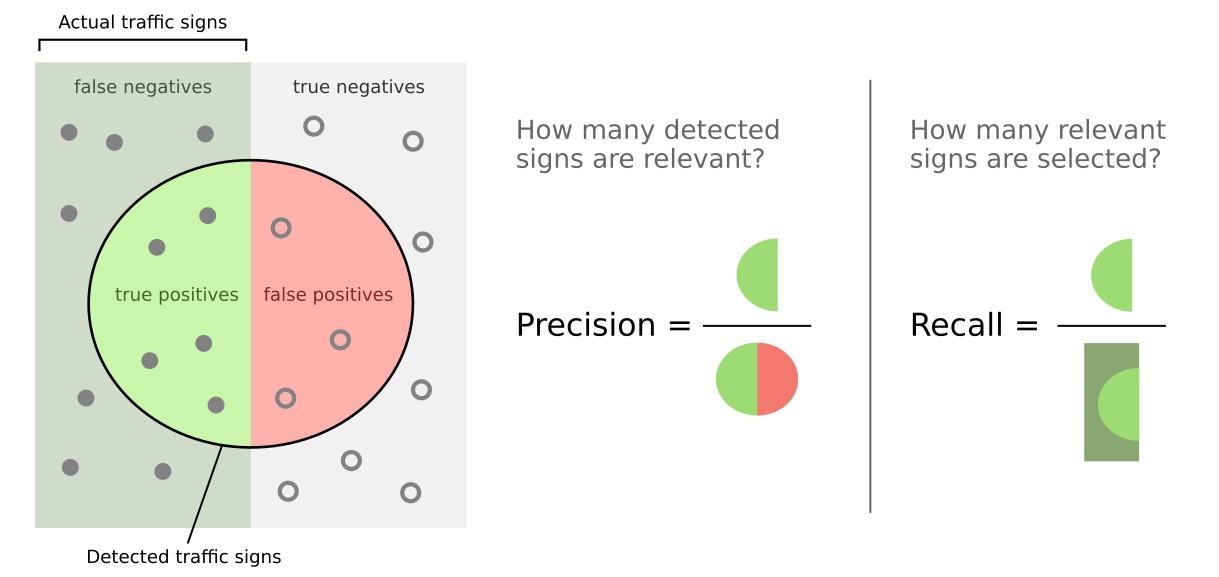
\includegraphics[width=0.8\linewidth]{figures/precisionrecall.png}
    \caption{Illustration of the precision and recall in the traffic sign detection context. Modified from \cite{wiki:precisionrecall}}
    \label{fig:precisionrecall}
\end{figure}{}

To get a perfect recall, one can detect everything, and so be sure not to miss any detection, but that will produce a lot of FP, decreasing the precision to very low values. Following the same idea, to get a perfect precision, one can detect only the one object it is most confident in, but that will result in very high FN and so low recall. This quick analysis shows the importance of correlating these two metrics to get meaningful results.

\subsection{Mean Average Precision}
\paragraph{}
Mean average precision, usually written as mAP, is the most used metric in object detection problem. This metric is more difficult to describe than the previous one, and is sometimes the subject of an entire paper by itself, for more information we advise you to consult \cite{wiki:metrics}.

As a quick description, mAP is the mean of the average precision (AP), which is computed for every classes. Average precision is the area under the curve of the recall vs precision graph where each point correspond to a confidence level. In other word, the AP is one if for any confidence level the recall and precision are equal to one.

Usual mAP is defined for a threshold of IoU with ground truth of $50\%$. But this research as well as lot of recent papers will use the notation $mAP@th$, where $th$ is the IoU threshold used to get the value of this metric. For example $mAP@50$ is the $mAP$ computed for detection matched with ground truth if they have an IoU higher than $50\%$.

\section{Conclusion}
\paragraph{}
Traffic sign detection and more broadly object detection have received a lot of attention from the research community over a large period of time. The rapid development of deep learning allowed great breakthroughs in this area, but the problem of getting similar level of accuracy real time on mobile devices is still largely unsolved. Improving the performance of the device is a solution to this problem, but optimization and fine-tuning is the key to achieve good results.



%%%%%%%%%%%%%%%%
% Chapter 2
%%%%%%%%%%%%%%%%

\chapter{Technical Approach} \label{chapter:technicalApproach}

\section{Introduction}
\paragraph{}
Running an accurate detection in real time on a smartphone is a difficult task as the literature review of Chapter \ref{litreview} already showed. Due to the limited time and scope of this work, we will not try to revolutionize this field, and focus on building on existing methods and taking advantage of the specificity of our task: traffic signs detection.

In this chapter we will first list the assumptions we took and expose their importance. We will then go deeper in the implementation by describing our output layer by showing its difference from other widely used networks and what are the benefit we are targeting with these changes. Once the output head is defined we will present our backbone structure and finish by detailing some implementation details such as the data management.

\section{Assumptions} \label{Assumptions}
\paragraph{}
Well known architectures for object detection, such as MobileNet-SSD \cite{sandler2018mobilenetv2}, already achieve great performance on mobile. It is out of scope of this work to improve over it for general object detection, but our task of object detection has some specificity that we can leverage to make things easier for detection. In this section we will present you those different assumptions and their motivations.

\subsection{Aspect ratio} \label{assumptionAspectRatio}
\paragraph{}
The first assumption we are going to take is that given a sign class, the aspect ratio of the object we are going to detect is always the same. Traffic signs follow well-defined standards, and if their size may change from one road condition to the other, their shape will stay the same. Due to perspective transformation they may appear with slightly different aspect ratio, but the sign giving information to the drivers, they are always facing it and so suffer from very small deformation when being seen from the windshield.

Neural network have already been proven to be very good at predicting the aspect ratio of the shape they are trying to detect. However, when using smaller backbone network, this prediction tend to become less accurate. This is often the case on models like tiny-yolo \cite{yolov3}. This makes us realize that the network spends a fair amount of effort computing those values accurately. Removing those completely will reduce significantly the complexity of the task while having only minor impact on the accuracy in our task.

\subsection{Position accuracy}
\paragraph{}
Following the same idea as during Section \ref{assumptionAspectRatio}, the accurate position is also something difficult to predict. Most of the detection networks, such as SSD \cite{liu2016ssd}, predict a given number of bounding boxes for an area, each having their own classes and position offset. Setting this position offset to the center of the detection area will make the task easier and reduce the load on the backbone network.

However, to maintain accuracy this requires to have smaller detection zone, showing an important trade-off here. Although this note is mostly important for deep backbone models that have a lot of convolution layers before the final output, having a small backbone network will mitigate this effect.

\subsection{Size accuracy}
\paragraph{}
Common one shot detection models like SDD \cite{liu2016ssd} and Yolo \cite{yolov3} use different layers to predict objects of different size. Each layers then predict variation around a given anchors size. Computation of Intersection over Union (IoU) with these default anchors showed that on our data, a small set of anchors achieved very high score. This allowed us to further reduce the complexity by removing the size prediction and directly use the anchor size as a prediction shape.

\subsection{Task complexity}
\paragraph{}
In addition to all the simplification given previously, we assume that our task is an easy case. Traffic sign are made to be easy to seen by human, they usually use bright colors and clear shapes. In addition, results from \cite{de1997road, janssen1993hybrid, besserer1993shape} show that simple pixel operation like color threshold and edges detection give good results on sign detection task. Showing us that a few layer backbone should perform great on this task.


\section{Detection layer}
\subsection{Intuition}
\paragraph{}
Following the assumptions given during Section \ref{Assumptions}, we are looking for a detection layer that is less generic than widely used ones, such as SSD \cite{liu2016ssd}. This loss should allow us to make the underlining function simpler and so easier to approximate with a neural network, which will allow us to use smaller network to approximate it.

Convolution operation are very good at doing pattern matching. Weights visualization techniques, such as the one presented in \cite{yosinski2015understanding} show that networks are very good at understanding the shape of an object. However, predicting the object size, even if possible as already done by different models \cite{yolov3, liu2016ssd, ren2015faster}, is a more complex process for this kind of operation.

Removing the need of this prediction is, however, not harmful to our traffic sign detection task, as explained in Section \ref{Assumptions}. Simplifying the task to classification of given bounding box regions of the images will strongly decrease the load on the backbone network complexity resulting in performance gain.

\subsection{Detection computation}
\paragraph{}
We chose to make our detection approach very similar to the one presented in SSD \cite{liu2016ssd}. We will predict classification and position of signs at different levels of our network and for each head each cell will predict one class.

Similarly, to the approach presented in \cite{liu2016ssd}, each output cell predict one bounding box with its class. This set of classes to predict also include the background in addition to the classes you want to detect to allow a common multi class classification setting with the use of a soft-max activation function on each cell.

However, our approach differs to the one they propose in that we do not choose between different anchors for each cell, and we do not predict the variation of shape and position around these anchors.

This modification leave us with a very light version of SSD, reduced to its core idea.

\subsection{Loss function}
\paragraph{}
The training objective we chose for this architecture is derived from the SSD training loss \cite{liu2016ssd}. We use here a very similar classification loss, based on soft-max loss for each cell.

\begin{align}
     Loss(x,c) = \sum_{i \in Pos} x_i - \sum_{i \in Neg} x_i
\end{align}{}
\[
    \text{with } Pos = \left\{ i | c_{i0} = 0 \right\} \text{ and } Neg = \left\{ i | c_{i0} = 1\right\}
\]

However, the imbalance between positive samples, $Pos$, and negative ones, $Neg$, is large so instead of relying on every sample we only select the most important negative one using the well know methods of hard negative mining. Instead of computing the loss on all the negative samples, we reduce it to the worst one, the one with the higher confidence. We choose here a $3:1$ negative to positive maximum ratio. This value have shown to prevent most of the negative predictions while not confusing the network on the detection task.

\subsection{Anchors}
\paragraph{}
To make detection easier, we pushed the concept of anchors forwards. The anchors are no longer base shape that the network can change. They are actual boxes that the network is forced to use for its prediction. This lead to a large loss of the general object detection task, but as we already discussed in this Chapter, this loss is acceptable in our case.

We selected a set of five different anchors, giving Intersection over Union (IoU) of $75.28\%$ in our ground truth data. Each anchor is predicted by a different head, the smaller anchors being predicted first in the network and the largest at the end, so they can take advantage of a larger activation area. The anchors we used during this study are given on Table \ref{tab:anchors}. More information about the anchors and how they are affected by the general architecture of the model is given on Chapter \ref{chapter:resutls}, Section \ref{sec:detectionLayerPos}.

\begin{table}[]
    \centering
    \caption{Anchors box chosen for detection}
    \begin{tabular}{|l|c|c|c|c|c|}
        \hline
        Anchors size & $3\times3$ & $5\times5$ & $7\times7$ & $12\times12$ & $21\times21$ \\
        \hline
    \end{tabular}
    \label{tab:anchors}
\end{table}{}

\section{Backbone}
\paragraph{}
This aspect of the the network will be more broadly covered in Chapter \ref{chapter:resutls}, where we are going to explain and justify all the different choices we made for this architecture. However, we are going to describe here the different building blocks we tried.
\subsection{Compute Block}
The main structure of the network is composed of stacked computation block. We explored different type of block during this study, and evaluated their computational efficiency by comparing their speed and accuracy. All the block share common property. They all use a ReLu6 \cite{sandler2018mobilenetv2} activation function, batch normalization \cite{ioffe2015batch} and dropout \cite{srivastava2014dropout}. The difference is on the way they do the internal computation.
\subsubsection{Convolution block}
The first type of block is the very basic 2D convolution, illustrated by Figure \ref{fig:convblock}. It is simple but have shown great results in the past and even if it has received multiple improvements, it is still a very good base line.
\subsubsection{Residual block}
The second block is a residual block \cite{szegedy2017inception}. Residual block allows to reduce much of the gradient vanishing problem, and so allows building a deeper network. This is not our goal here as we want to maintain a small size, but this could improve training efficiency at a minimal cost. This block is illustrated in Figure \ref{fig:resblock}.
\subsubsection{Inverted residual Bottleneck}
The Inverted residual Bottleneck block was introduced by MobileNetv2 \cite{sandler2018mobilenetv2} as structure tailored to run on mobile devices. It is composed of a first expansion layer, a 2D convolution with kernel $(1,1)$, followed by a depth wise 2D convolution with kernel $(3,3)$, and the final outcome is given by projection layer, a 2D convolution with $(1,1)$ kernel. All of that are bundled in a residual block. A graphical representation of this block, From MobileNet v2 paper \cite{sandler2018mobilenetv2}, is provided on Figure \ref{fig:invertedbottleneckblock}.

\begin{figure}
  \begin{center}
    \begin{subfigure}[t]{.24\linewidth}
      \centering
      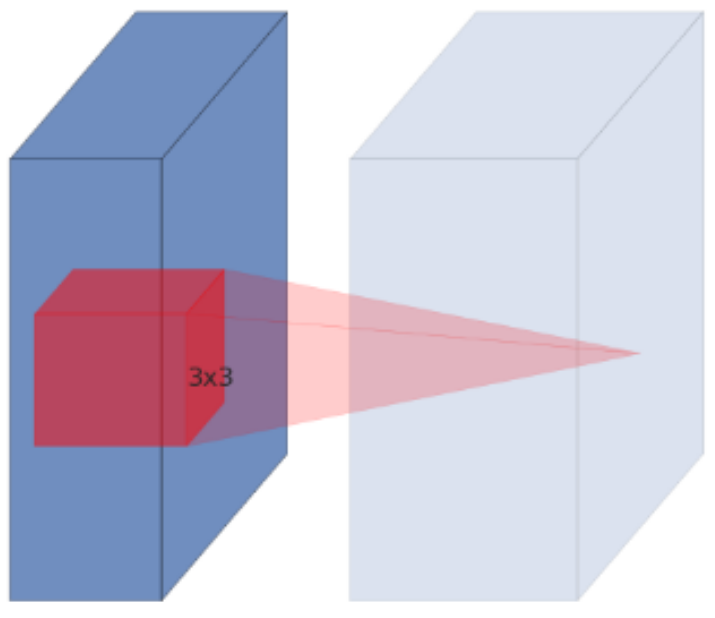
\includegraphics[width=.8\linewidth]{figures/mobilenetv2_conv.png}
      \caption{2D Convolution block}
      \label{fig:convblock}
    \end{subfigure}
    \begin{subfigure}[t]{.24\linewidth}
      \centering
      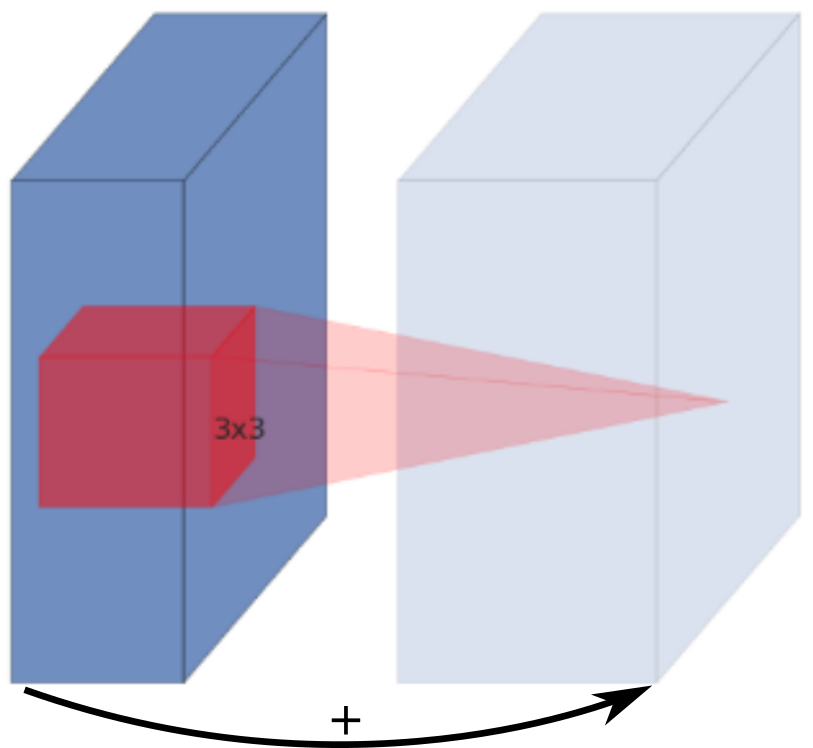
\includegraphics[width=.8\linewidth]{figures/mobilenetv2_resnet.png}
      \caption{Residual convolution block}
      \label{fig:resblock}
    \end{subfigure}
    \begin{subfigure}[t]{.5\linewidth}
      \centering
      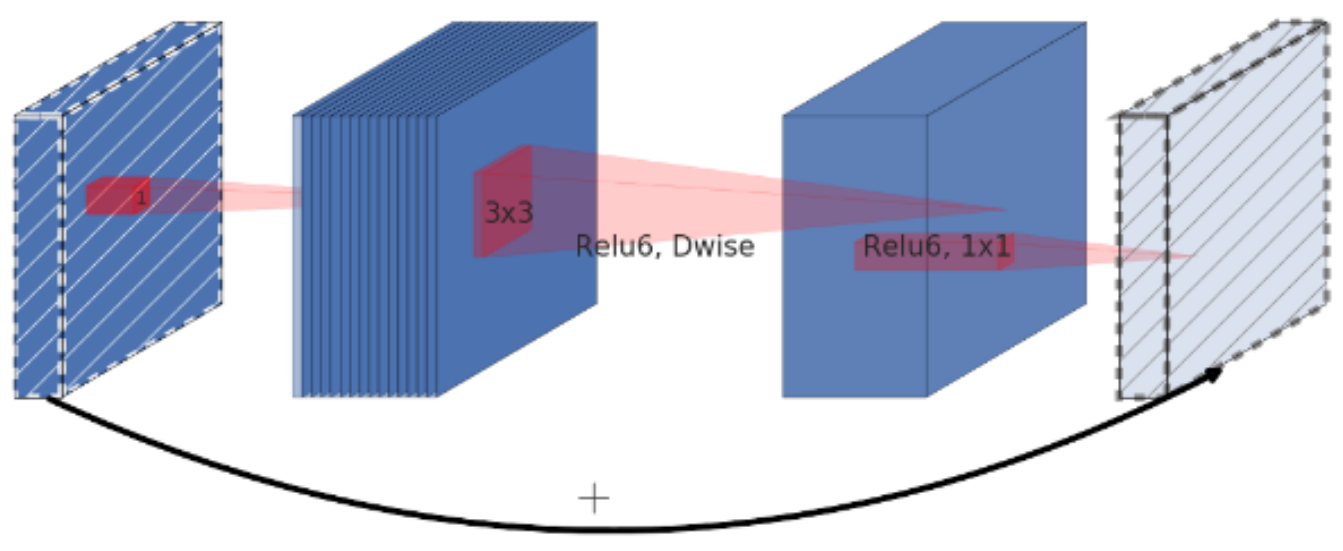
\includegraphics[width=.99\linewidth]{figures/mobilenetv2_inverted_residual_botleneck.png}
      \caption{Inverted residual block \cite{sandler2018mobilenetv2}}
      \label{fig:invertedbottleneckblock}
    \end{subfigure}
    \caption{Graphical representation of the different block used in this study, Illustrations from MobileNet V2 paper \cite{sandler2018mobilenetv2}}
  \end{center}
\end{figure}


\section{Training}
\subsection{Classes}
\paragraph{}
Our architecture is capable of being trained for multiple sign class, but in the context of this project we are mainly interested in one class, US diamond warning signs. Some example of such signs are available on Figure \ref{signExample}.

\begin{figure}
  \begin{center}
    \begin{subfigure}[t]{.3\linewidth}
      \centering
      
\includegraphics[height=0.8\linewidth]{figures/W1-1_R.jpg}
      \caption{W1-1}
    \end{subfigure}
    \begin{subfigure}[t]{.3\linewidth}
      \centering
      
\includegraphics[height=0.8\linewidth]{figures/W1-3_L.jpg}
      \caption{W1-3}
    \end{subfigure}
    \begin{subfigure}[t]{.3\linewidth}
      \centering
      
\includegraphics[height=0.8\linewidth]{figures/W1-4_L.jpg}
      \caption{W1-4}
    \end{subfigure}
    \caption{Example of US diamond warning signs, with there MUTCD sign class.}
    \label{signExample}
  \end{center}
\end{figure}

We chose not to aggressively ask the network to classify each sign directly into there MUTCD code as this task is much more difficult than only detection and can be handled with more accuracy by a specialized network. In addition, this strategy allow to reduce the input size. This smaller input size may make it impossible even for human to tell which MUTCD class the sign is, but is enough to say that there is a sign there, which is what we care about in this work. Once the sign is detected the image can be cropped at full resolution and given to a classification algorithm.

This approach may look very similar to the region proposal network of RCNN \cite{girshick2014rich}, and it is when you use only one class. However, when other classes are added this similarity get less clear. For example, you may want to add a stop sign class that does not require any other processing, or a speed limit class that will require specific digit detection algorithm.

\subsection{Data} \label{data_pres}
\paragraph{}
During this research, a large variety of data have been used. All this data were manually annotated by our research team and may be the subject of a later publication. The image were collected using either smartphone mounted on the windshield or externally mounted high resolution camera. Most of the images were collected in the north of the state of Georgia or around Nashville, over a large period of time.

This data set contains a large variety of  luminosity conditions and different seasonal background changes. However, it is important to note that this data set does not cover all the possible cases. First in the data collection regions, most of the rural areas are populated by trees, which represents most of the background of our images. In addition, the image collection was not the main purpose of the trip to those rural areas. As a result certain weather conditions such as rain are not widely present in the data. Data augmentation and generalization capabilities of the network may allow us to overcome such limitations, but without good testing data it would be difficult to assess those.

More information about the data are given in Appendix \ref{data}.

\subsection{Data generation} \label{sec:dataGen}
\paragraph{}
The data presented in Section \ref{data_pres} is a great source of information and are very important to this study, but they do not have enough samples to train a new model end to end correctly. To solve that issue we decided to rely on generating artificial data.

Our goal on this task was not to get photo realistic data, as they are not very realistic at very low resolution as we plan to use here, and are not needed. We want the network to use this data to get a broad understanding of what it should look for, on a very generic basis. To meet this goal we chose to train our model to detect yellow squares rotated by $45\deg$. The data we generate to meet this goal are far from any realistic image or even the real traffic sign we want to detect. An example of the generated image is given on Figure \ref{fig:fake_im_ex}. These images are generated following a very simple procedure, first the background is set to average pixel value of the real dataset from Section \ref{data_pres}. Then $500$ random polygons are drawn on top of it, starting with big ones and getting smaller and smaller. These polygons are convex and have between three and ten vertices. They are sampled by randomly choosing the angle and distance of each vertex regarding the center, while the color is randomly sampled from the color distribution observed in the real dataset. The goal of this generation is to create lot of different edges of similar color as in real live and to provide a not flat background to the target shapes. Over this background are then added the rotated yellow squares. Five such shape are added on each image, their sizes are sampled from the anchors size of the model, and colors are sampled following a normal distribution centered on yellow. The centers of the shapes are selected not to have large overlap with the edges of the image and to prevent any overlapping on each other. To prevent the model to learn to detect yellow objects we then add three not rotated square that otherwise follow the same logic as previously.

\begin{figure}
    \centering
    
\includegraphics[width=0.5\linewidth]{figures/fake_data_ex.jpg}
    \caption{Example of artificially generated data}
    \label{fig:fake_im_ex}
\end{figure}{}

Using this logic we generated $20,000$ images and annotations to be used for our experiments.

\paragraph{}
We also considered replacing this pretraining data by a first training on a classification task. But we finally considered this step as not bringing enough benefit. First because training on sign classification will not bring much help as it will just teach the network to focus on the pictograph in the sign, not the sign itself. In addition, we could have used more generic dataset such as CIFAR 10 \cite{krizhevsky2009cifar10}, but we considered our model to be too shallow to learn useful features from such a training. The fact that the prediction is computed at different layers was also a problem to that idea. In conclusion, we decided that a first training on a classification task would not bring as much improvement as artificially generated data could.


\subsection{Data augmentation and prepossessing}
\paragraph{}
As it is common in deep learning, overfitting often arise on large networks. There is many different ways to prevent that. Some directly in the network, such as dropout \cite{srivastava2014dropout} that disable some connections in the network during training, or batch normalization \cite{ioffe2015batch} that normalize the output of each layer, improving training speed and mitigating the effects of overfitting. 

We applied these two methods to our network, but it is not enough to skip data augmentation entirely. Data augmentation was done using the classical approach, linear transformation of the image. This random transformation changes the image by applying random zoom in/out, shift and vertical symmetries. Rotation and shear were excluded from the data augmentation as they may result in change of the bounding box shape that depends on the actual object shape is are hard to predict. We also applied a color transformation to the image, by changing the brightness in order to simulate different lighting conditions.

\subsection{Architecture search}
\paragraph{}
In Chapter \ref{architectureSearch}, we presented different strategies to perform architecture search. Because of the lack of public implementation of this type of optimization strategy, and because of the size of our model, we chose to go for a broader way to explore meta-parameters. We used the classical grid search approach to this problem. As our model is able to be trainned in about an hour, such an approach does not cause any problem.

We used this the same way as NetAdapt \cite{yang2018netadapt} to fine tune the global architecture defined previously. This approach allowed us to get the relevant number of filters of each layer as well as tuning the dropout strategy to use.

In addition, similarly to ENAS \cite{pham2018efficient}, we implemented a parameters sharing process, allowing to save a lot of time on some grid search tasks.



%%%%%%%%%%%%%%%%
% Chapter 3
%%%%%%%%%%%%%%%%

\chapter{Results} \label{chapter:resutls}

\section{Exploring model architecture}
\subsection{Introduction}
\paragraph{}
During this study we explored different way to build an efficient architecture for our task. This process required a lot of trial and measurement. The goal of this section is to illustrate and explain the different choice made during the choice of the final architecture. In this optic we will cover different topic, starting with the choice of the input size, followed by the position of the detection layers, and we will then explore the details of the feature extraction part of the network.

\subsection{Input size} \label{sec:inputSize}
\paragraph{}
During this study we explored different input resolution to run our model. This point is the most critical point in our study, as we mainly focus on speed. It is expected that the number of computation needed by a fully convolutional architecture such as the one we use here is linearly correlated to the input size. This linearity can be observed on Figure \ref{fig:latencysize}. But at the same time, the lower the resolution of the image, the less information are available to allow detection. This is particularly true for small sign that may become invisible. However, our study use case allow such sign not to be very accurately detected as they will get bigger as the car move closer to them.

We choose to keep the original image aspect ratio recorded by smartphone camera to maintain the semantic as the one human are used to, reducing also the deformation created by small rotation of the objects and keeping the symmetry of the information loss on both axis. From that we explored different size to see if they are good enough for a human to use. Figure \ref{resizeExample} show clear example of this. As you can see, the scaling induce a lot of information loss, but the information remaining is still enough for a human being to spot the sign on the image, leading to believe that a convolutionnal neural network can perform the same operation.

\begin{figure}
  \begin{center}
    \begin{subfigure}[t]{.49\linewidth}
      \centering
      
\includegraphics[width=0.99\linewidth]{figures/im_example_full.jpg}
      \caption{Full resolution image, $1080\times1920$}
    \end{subfigure}
    \begin{subfigure}[t]{.49\linewidth}
      \centering
      
\includegraphics[width=0.99\linewidth]{figures/im_example_440x800.jpg}
      \caption{Image resized at $440\times800$}
    \end{subfigure}
    \begin{subfigure}[t]{.49\linewidth}
      \centering
      
\includegraphics[width=0.99\linewidth]{figures/im_example_220x400.jpg}
      \caption{Image resized at $220\times400$}
    \end{subfigure}
    \begin{subfigure}[t]{.49\linewidth}
      \centering
      
\includegraphics[width=0.99\linewidth]{figures/im_example_110x200.jpg}
      \caption{Image resized at $110\times200$}
    \end{subfigure}
    \caption{Example of an image resized at different size and displayed at same size. This image contains two signs, one on the foreground, clearly visible, and another one at the level of the forest in the background. This second one is clearly visible on a full screen image at full resolution, but quickly disappear as resolution drop, while the bigger one stay clear.}
    \label{resizeExample}
  \end{center}
\end{figure}

\begin{figure}
  \begin{center}
    \begin{subfigure}[t]{.49\linewidth}
      \centering
      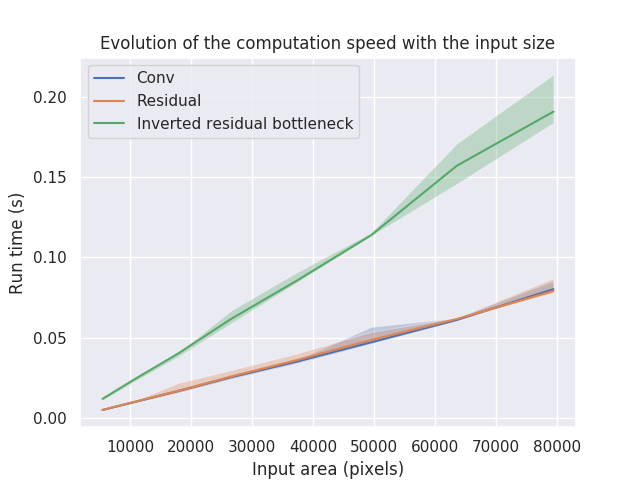
\includegraphics[width=0.99\linewidth]{figures/speed_by_nn_size_and.png}
      \caption{Latency evolution with input size}
      \label{fig:latencysize}
    \end{subfigure}
    \begin{subfigure}[t]{.49\linewidth}
      \centering
      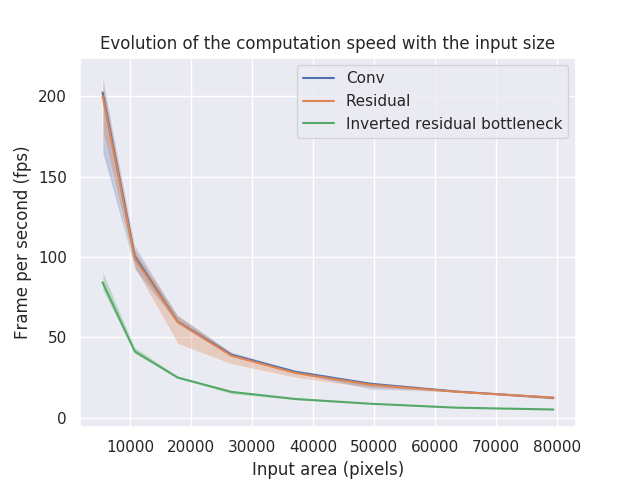
\includegraphics[width=0.99\linewidth]{figures/speed_by_nn_size_fps_and.png}
      \caption{FPS evolution with input size}
      \label{fig:fpssize}
    \end{subfigure}
    \caption{Evolution of the prediction speed for different block type. The input area represent the number of pixel in the input image. These results were obtained by running a TensorFlow Lite version of the model on Samsung S6 (SM-920T) on one thread. The hard line represent the average value, while the area go from the minimum to the maximum value over all runs.}
    \label{resizeExample}
  \end{center}
\end{figure}

% add experiment about the size / accuracy ?
We first experimented with image at $220\times400$ resolution, however, as the accuracy was good we decided to step down to $110\times200$. This smaller resolution also gave us a good accuracy while reducing the number of computation by a factor $4$.

\subsection{Detection layers position} \label{sec:detectionLayerPos}
\paragraph{}
The layers doing the detection of the signs are located at two different position of the network. This to allow more local features to be taken into account for small object while larger object have a larger activation area.

A statistical analysis of our dataset performed following the same idea as in \cite{yolov3}. We chose to use five different anchors. These anchors are given in Table \ref{tab:anchors}. This set of anchors give us an average IoU over our dataset of $75.28\%$, showing the drawback of the assumption chosen previously, but also showing that they are valid if you do not want perfect boxes. This anchors boxes are completely compatible with the activation area there corresponding layers as displayed on Table \ref{tab:activationArea}.

Because of the assumption we chose in Chapter \ref{chapter:technicalApproach}, Section \ref{Assumptions}, the number of bounding boxes our model can predict is limited and have given position. These boxes depend on multiple factor, the anchor size, but also the general architecture of the backbone network as well as the input size. Figure \ref{fig:anchors} represent all the different box our model can predict, displaying clearly the limit of our assumptions in term of accuracy, but giving enough coverage of the space to provide good results.

\begin{figure}
  \begin{center}
    \begin{subfigure}[t]{.49\linewidth}
      \centering
      
\includegraphics[width=0.99\linewidth]{figures/anchors/boxes_layers_0.png}
      \caption{Every possible boxes for anchor $3\times3$}
    \end{subfigure}
    \begin{subfigure}[t]{.49\linewidth}
      \centering
      
\includegraphics[width=0.99\linewidth]{figures/anchors/boxes_layers_1.png}
      \caption{Every possible boxes for anchor $5\times5$}
    \end{subfigure}
    \begin{subfigure}[t]{.49\linewidth}
      \centering
      
\includegraphics[width=0.99\linewidth]{figures/anchors/boxes_layers_2.png}
      \caption{Every possible boxes for anchor $7\times7$}
    \end{subfigure}
    \begin{subfigure}[t]{.49\linewidth}
      \centering
      
\includegraphics[width=0.99\linewidth]{figures/anchors/boxes_layers_3.png}
      \caption{Every possible boxes for anchor $12\times12$}
    \end{subfigure}
    \begin{subfigure}[t]{.49\linewidth}
      \centering
      
\includegraphics[width=0.99\linewidth]{figures/anchors/boxes_layers_4.png}
      \caption{Every possible boxes for anchor $21\times21$}
    \end{subfigure}
    \caption{Graphical representation of all the possible boxes that the network can predict, displayed per anchor. This illustration considers an input shape of $110\times200$ pixels, and the model architecture described in Table \ref{tab:nnstruct}.}
    \label{fig:anchors}
  \end{center}
\end{figure}


\subsection{Feature Extraction}
\paragraph{}

As we already discussed during Section \ref{Assumptions}, the traffic signs are made to be detected and are so very easy to capture. As you can see on Table \ref{tab:nnstruct} and Figure \ref{fig:nnstruct}, the features extraction layers is very limited compared to other lightweight models such as MobileNet \cite{sandler2018mobilenetv2}. With only five layers as a first feature extraction followed by three layers of higher order feature detection. This architecture allows reducing drastically the number of floating-point operation needed. Our model requires $39$ Millions floating-point operation (FLOP), while common architecture like tiny Yolo v3 \cite{yolov3} use $5,600$ Millions FLOP.

\begin{table}[]
    \centering
    \caption{Description of the neural network structure, block by block, giving the link between the blocks and some information such as the use Batch Normalization (BN) or residual connections (Res).}
    \begin{tabular}{|c|c|c|c|c|c|c|c|c|}
    \hline
    Name & Filter & Kernel & Stride & Activation & BN & Res & Input size & Input \\ \hline
    Conv1 & $8$ & $(3, 3)$ & $(2, 2)$ & ReLu6 & \checkmark &  & $(111, 201, 3)$ &  \\
    block\_0 & $8$ & $(3, 3)$ & $(1, 1)$ & ReLu6 & \checkmark & \checkmark & $(55, 100, 8)$ & Conv1 \\
    block\_1 & $16$ & $(3, 3)$ & $(2, 2)$ & ReLu6 & \checkmark &  & $(55, 100, 8)$ & block\_0 \\
    block\_2 & $16$ & $(3, 3)$ & $(1, 1)$ & ReLu6 & \checkmark & \checkmark & $(28, 50, 16)$ & block\_1 \\
    block\_3 & $16$ & $(3, 3)$ & $(1, 1)$ & ReLu6 & \checkmark & \checkmark & $(28, 50, 16)$ & block\_2 \\
    block\_4 & $16$ & $(3, 3)$ & $(2, 2)$ & ReLu6 & \checkmark &  & $(28, 50, 16)$ & block\_3 \\
    block\_5 & $16$ & $(3, 3)$ & $(1, 1)$ & ReLu6 & \checkmark & \checkmark & $(14, 25, 16)$ & block\_4 \\
    block\_6 & $16$ & $(3, 3)$ & $(1, 1)$ & ReLu6 & \checkmark & \checkmark & $(14, 25, 16)$ & block\_5 \\
    output\_1 & $2$ & $(3, 3)$ & $(1, 1)$ & Linear &  &  & $(28, 50, 16)$ & block\_3 \\
    output\_2 & $2$ & $(3, 3)$ & $(1, 1)$ & Linear &  &  & $(28, 50, 16)$ & block\_3 \\
    output\_3 & $2$ & $(3, 3)$ & $(1, 1)$ & Linear &  &  & $(14, 25, 16)$ & block\_6 \\
    output\_4 & $2$ & $(3, 3)$ & $(1, 1)$ & Linear &  &  & $(14, 25, 16)$ & block\_6 \\
    output\_5 & $2$ & $(3, 3)$ & $(1, 1)$ & Softmax &  &  & $(14, 25, 16)$ & block\_6 \\
    \hline
    \end{tabular}
    \label{tab:nnstruct}
\end{table}{}


\begin{table}[]
    \centering
    \caption{Activation area and associated anchors of each output layers}
    \begin{tabular}{|c|c|c|}
        \hline
        Layer & Anchors size & Activation area \\ \hline
        output\_1 & 3 & $24\times24$ \\
        output\_2 & 5 & $24\times24$ \\
        output\_3 & 7 & $56\times56$ \\
        output\_4 & 12 & $56\times56$ \\
        output\_5 & 21 & $56\times56$ \\
        \hline
    \end{tabular}
    \label{tab:activationArea}
\end{table}{}

\begin{figure}
    \centering
    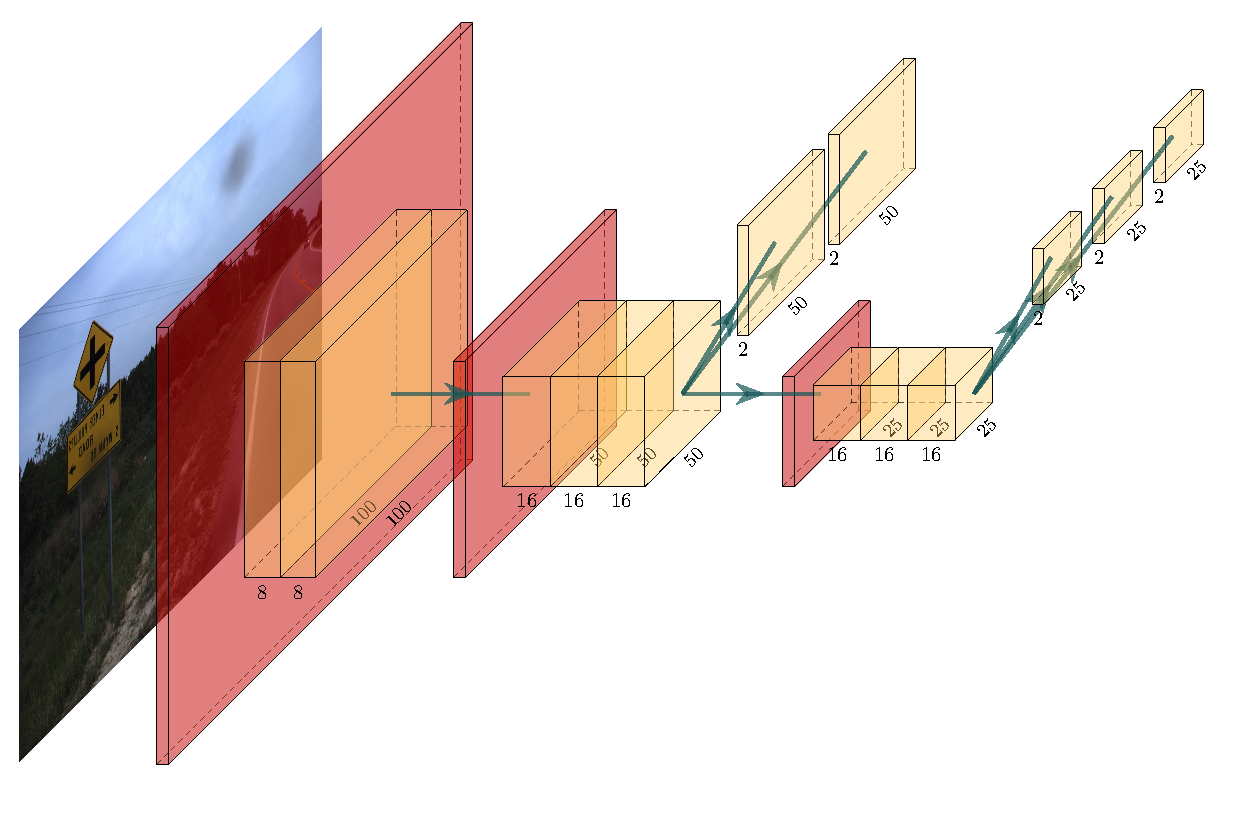
\includegraphics[width=\linewidth]{figures/my_arch}
    \caption{Structure of the neural network, orange boxes are convolution, red boxes indicate a stride 2 on the following layer}
    \label{fig:nnstruct}
\end{figure}{}

\section{Overfitting study} \label{sec:overfit}
\paragraph{}
A first basic check to verify if the model can learn something usefully is to try to overfit it on the data you have. If the model is not capable of overfitting them, then your model is not complex enough to understand the complexity of the data. The idea is that if the network is not able to give correct prediction on the training set, how can we expect it to give correct prediction on unseen data.

We performed this kind of study for the three different kind of block we consider here: inverted residual bottleneck, residual and convolution, as well as for three different set of filters size: $(32,64)$, $(16,24)$ and $(8,16)$. The first number representing the number of filters for Conv1 and Block 0, while the second number being the number of filters for block 1 to 6. Please refer to Table \ref{tab:nnstruct} for more information about those layers. All the block considered here are supposed to have similar expression potential, however, using different number of filters as a big impact on how much information the network can carry. On a general basis, the more filters the network has, the easier it will be to overfit the data.

To perform this analysis, we set the experiment in the following way. Aside from the parameters given previously, all the other meta parameters are set to same values across all test. The data augmentation is disabled, and the dropout is set to $0$. No early stopping strategy is used, and all network are trained for $200$ epochs on the full training split of the dataset, with a batch size of $128$.

\begin{figure}
  \begin{center}
    \begin{subfigure}[t]{.49\linewidth}
      \centering
      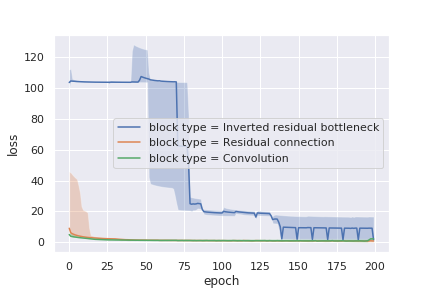
\includegraphics[width=0.99\linewidth]{figures/all_epoch_loss_block_type.png}
      \caption{Evolution of the training loss with epoch, for different block type}
      \label{fig:overfitloss}
    \end{subfigure}
    \begin{subfigure}[t]{.49\linewidth}
      \centering
      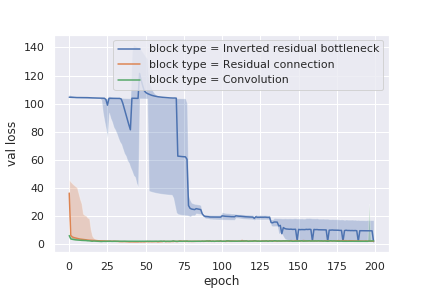
\includegraphics[width=0.99\linewidth]{figures/all_epoch_val_loss_block_type.png}
      \caption{Evolution of the validation loss with epoch, for different block type}
      \label{fig:overfitvalloss}
    \end{subfigure}
    \begin{subfigure}[t]{.49\linewidth}
      \centering
      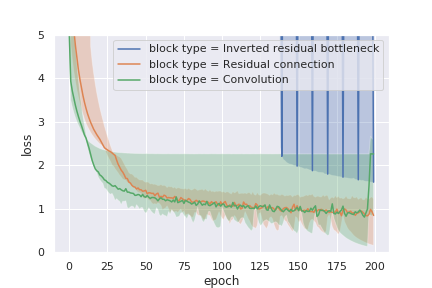
\includegraphics[width=0.99\linewidth]{figures/all_epoch_loss_block_type_zoomed_0_5.png}
      \caption{Evolution of the training loss with epoch, for different block type, zoomed on loss between 0 and 5}
      \label{fig:overfitloss_zoom}
    \end{subfigure}
    \begin{subfigure}[t]{.49\linewidth}
      \centering
      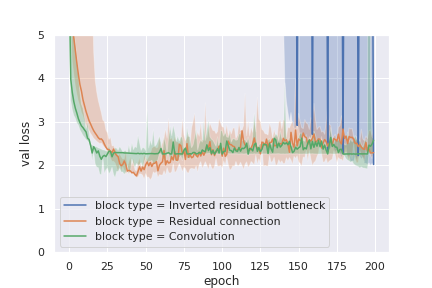
\includegraphics[width=0.99\linewidth]{figures/all_epoch_val_loss_block_type_zoomed_0_5.png}
      \caption{Evolution of the validation loss with epoch, for different block type, zoomed on loss between 0 and 5}
      \label{fig:overfitvalloss_zoom}
    \end{subfigure}
    \caption{Evolution of the validation and training loss for different block type, the hard line represent the median value, while the highlighted area go from the min to the max, for the different filters count.}
    \label{fig:overfit}
  \end{center}
\end{figure}

The training curve we get from this experiment are displayed on Figure \ref{fig:overfit}. You can see on Figure \ref{fig:overfitloss} and \ref{fig:overfitvalloss} that one block have lot of trouble learning anything. The inverted residual bottleneck block show very chaotic loss evolution, and never manage to overfit the data. As displayed on Figure \ref{fig:overfitloss_zoom}, the training loss of this block never reach $1.5$ in the given $200$ epochs. In the worst case, this block never get train loss better than $5$, while mAP@0.5 for loss over $3$ in this setup never crossing the bar of the $0.03$. On the other hand, Figure \ref{fig:overfitvalloss_zoom}, show that in this region of the graph the validation loss of the inverted residual bottleneck block in very consistent with the training loss, we are going to come back to that point latter.

The two other kinds of blocks, convolution and residual, behave in a similar manner. In both case their loss quickly drop to values around $2$ and overfitting start to appear. Overfitting is clearly visible for the residual block around epoch $40$ on Figure \ref{fig:overfitvalloss_zoom}. Both show that they successfully overfit the dataset, expect the case of the convolution block with the smaller filters, which did not manage to overfit the data, resulting in a steady loss at $2.3$, visible on Figure \ref{fig:overfitloss_zoom}.

\paragraph{}
The case of the inverted residual bottleneck block catch our attention, for multiple reason. First, the case getting the best results is not the one with the higher number of filters as one could expect, but the one with the smallest number of filters. In addition, even with all the trick supposed to prevent overfitting disabled, the network still did not overfit and get consistently decreasing training and validation loss. We decided to train it further, running for $600$ with some data augmentation and dropout to prevent overfitting. The evolution of the loss can be seen on Figure \ref{fig:mn600}. You can see that as previously, in Figure \ref{fig:overfit}, this model as a strange behavior during the first epochs, until a point where the loss start dropping in a more usual fashion. Training could have been performed for a longer time as the loss was still decreasing, but that first exploration showed encouraging results with an mAP@50 reaching $0.4$. However, as you can see on figure \ref{fig:overfitmAP}, this mAP level on the validation set is reached by all the different block even when trying to overfit them on the training data.

\begin{figure}
  \begin{center}
    \begin{subfigure}[t]{.49\linewidth}
      \centering
      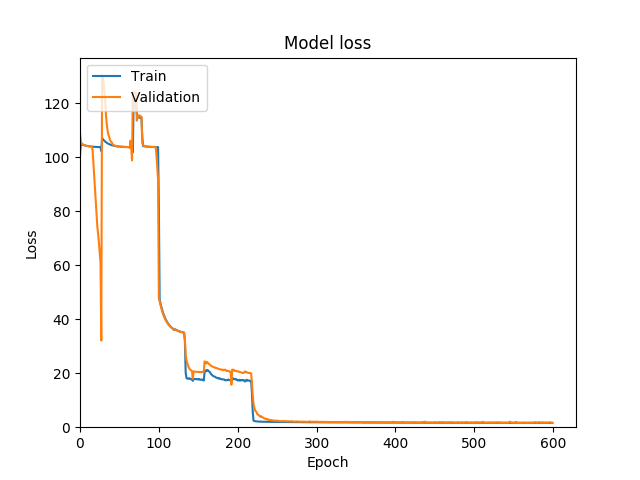
\includegraphics[width=0.99\linewidth]{figures/nNetloss_mn_816_600.png}
      \caption{Evolution of the loss with epochs}
      \label{fig:mn600loss}
    \end{subfigure}
    \begin{subfigure}[t]{.49\linewidth}
      \centering
      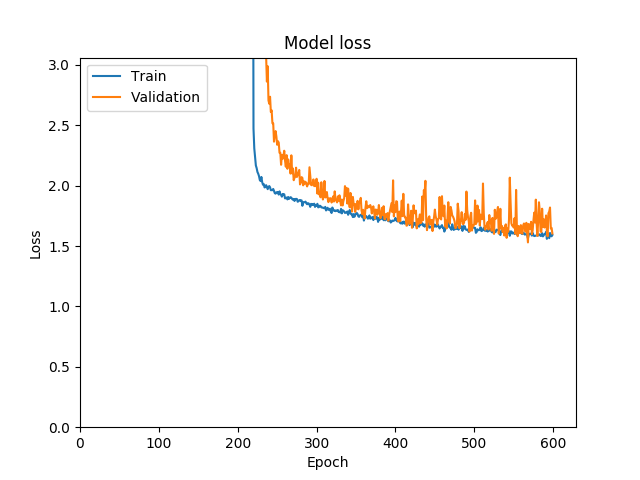
\includegraphics[width=0.99\linewidth]{figures/nNetloss_mn_816_600_zoomed.png}
      \caption{Evolution of the loss with epochs, zoomed on y axis}
      \label{fig:mn600lossZoomed}
    \end{subfigure}
    \caption{Evolution of the validation and training loss during training for an inverted residual bottleneck block type model, trained over $600$ epochs.}
    \label{fig:mn600}
  \end{center}
\end{figure}

\begin{figure}
    \centering
    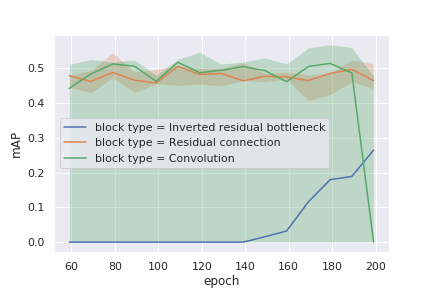
\includegraphics[width=.5\linewidth]{figures/all_epoch_mAP_block_type.png}
    \caption{Evolution of the mAP@50 on validation set for the different blocks type during the overfiting study.}
    \label{fig:overfitmAP}
\end{figure}{}

\paragraph{}
From this study we concluded that the inverted residual bottleneck can be difficult to train and does not provide better accuracy than what the other block propose. In the other hand as expected convolution and residual convolution perform in a quite similar way as expected, with the residual version looking more stable even if slower to train. From these results we chose to focus our efforts toward the residual block, discard any more exploration on the convolutions block, and keep the inverted residual bottleneck as a comparison for the rest of the study.

\section{Pretraining}
\paragraph{}
Study of the weights trained during Section \ref{sec:overfit} showed that the trained network were still performing in a sub-optimal fashion. Weights of the first layer filters were still very noisy and no matter the training strategy used remained so. If they still have interest on yellow objects, most of them were still random and very far from the edge detector filters one would expect from a properly trained network.

The most common way to solve that issue is to have more data for training. When having more training samples is not an option, the usual way is to pretrain the model on one of the public dataset, such as ImageNet \cite{deng2009imagenet} or Cifar \cite{krizhevsky2009cifar10}. But if such a strategy have been proven to be successful to get good generic first filters and if this method would probably have been successful in this study too, the filters would have been generic and so not as efficient as possible for this task, resulting in more filters than necessary. Our main goal being to target efficiency we chose another approach to that problem. As already described in Section \ref{sec:dataGen}, we chose to generate new artificial data to train the network on a similar task.

For this new task, being easier and virtually having unlimited data available, it was easy to achieve over $0.8$ mAP@50 on this set of data with all the different models. Using this trained weights for fine-tuning on real world data, successfully boosted the accuracy of our model, adding from $0.1$ to $0.2$ to the final mAP, as you can see on Table \ref{tab:mapFineTuning}. This Table compare different models, with different filters, each described by a tuple of two numbers. The first representing the number of
filters for Conv1 and Block 0, while the second being the number of filters for block 1 to 6. The Table compare the models for two different intersection over union thresholds, $25\%$ and $50\%$, to give a better idea of there localization accuracy, and give the relative improvement obtained by training first on the artificial data before fine-tuning on the real cases. For each model the same meta parameters were used during training. In the direct training case, the models were trained for $600$ epochs on the real data starting with random weights with an initial learning rate of $0.01$. In the fine-tuning case, the models were first trained for $200$ epochs on the artificial data, with an initial learning rate of $0.01$, and these weights were then used for training for $600$ epochs on the real world data with a smaller initial learning rate of $0.001$. Table \ref{tab:mapFineTuning} clearly show that using the artificially generated data provide a large improvement in accuracy as well as allowed to stabilize the training process preventing case like the residual model with filters $(16,24)$ not being able to learn anything over the training. As previously experienced during this study, the inverted residual bottleneck also behave here strangely. If once again we cannot say that this layer is not working, initializing the weights on the artificial data did not bring any improvements and even make results worst.

\begin{table}[]
    \centering
    \caption{Summary of the evolution of the mAP with and without fine turning. Direct training values are get after training random weights on the real word annotation, while Fine tuning are get by first training the weights on artificial data.}
    \begin{tabular}{|c|c|c|c|c|c|c|c|}
        \hline
        \multirow{3}{*}{Block type} & \multirow{3}{*}{Filters} & \multicolumn{4}{|c|}{mAP} & \multicolumn{2}{|c|}{\multirow{2}{*}{Improvement}} \\
        & & \multicolumn{2}{|c|}{Direct Training} & \multicolumn{2}{|c|}{Fine tuning} & \multicolumn{2}{|c|}{}\\ 
        & & @25 & @50 & @25 & @50 & @25 & @50 \\ \hline
        \multirow{3}{*}{Residual} & $(8,16)$   & $0.58$ & $0.45$ & $0.68$ & $0.55$ & $+17.2\%$ &                               $+22.2\%$ \\
                                  & $(16,24)$ & $0.00$ & $0.00$ & $0.73$ & $0.61$ & $+\infty$ & $+\infty$ \\
                                  & $(32,64)$ & $0.62$ & $0.52$ & $0.82$ & $0.67$ & $+32.3\%$ & $+28.8\%$ \\ \hline
        Inverted Residual         & $(8,16)$   & $0.49$ & $0.38$ & $0.43$ & $0.30$ & $-12.24\%$ &                               $-21.05\%$\\ \hline
    \end{tabular}
    \label{tab:mapFineTuning}
\end{table}


As you can see the accuracy vary a lot from one model to the other, but as always in this study, it is always a matter of trade of. More filters mean more computation done which, on mobile device, automatically results in higher latency. With a previous demonstration of that showed on Figure \ref{fig:latencysize}, where you can see that the latency is directly linked to the input size, showing the importance of the meta parameters in the final detection speed.

\section{Latency study}
\paragraph{}
Speed is the ultimate target of this study, it has been under all the assumption and decision we took, but so far we barely discussed or gave results to asses these choices. The goal of this section is to expose the parameters having the more importance for over detection speed in our model and how they also affect accuracy. We are going here to cover the more important one, such as filter size and block type, input size being already discussed in Section \ref{sec:inputSize}.

\begin{figure}
  \begin{center}
    \begin{subfigure}[t]{.49\linewidth}
      \centering
      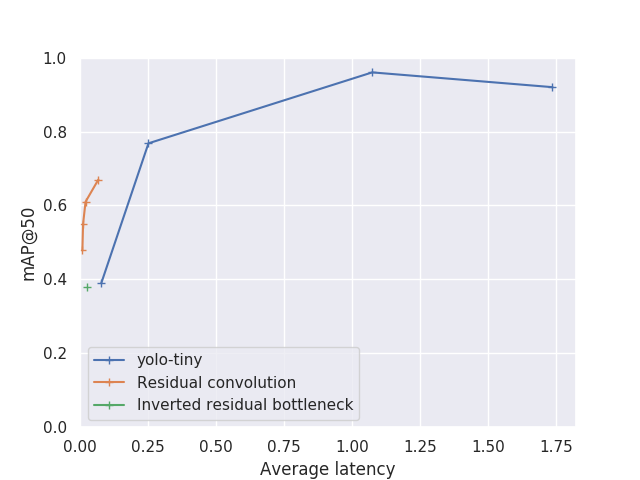
\includegraphics[width=0.99\linewidth]{figures/map_at_50_latency_models.png}
      \caption{Evolution of the mAP@50 with the latency}
    \end{subfigure}
    \begin{subfigure}[t]{.49\linewidth}
      \centering
      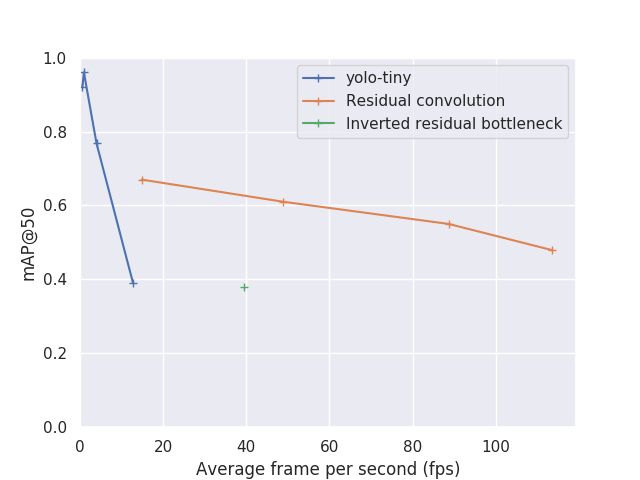
\includegraphics[width=0.99\linewidth]{figures/map_at_50_fps_models.png}
      \caption{Evolution of the mAP@50 with the frame per second}
    \end{subfigure}
    \begin{subfigure}[t]{.49\linewidth}
      \centering
      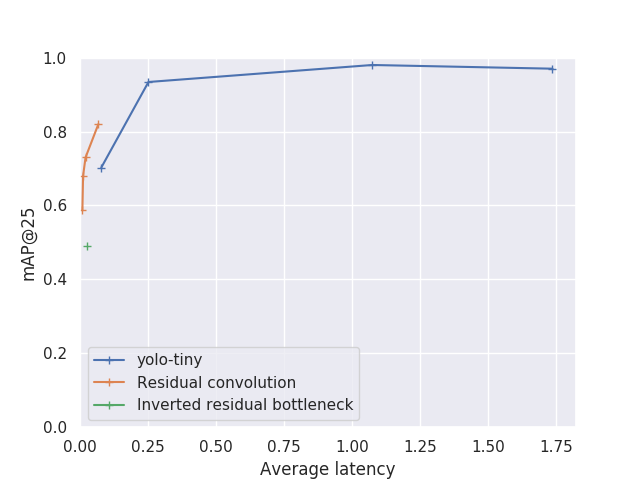
\includegraphics[width=0.99\linewidth]{figures/map_at_25_latency_models.png}
      \caption{Evolution of the mAP@25 with the latency}
    \end{subfigure}
    \begin{subfigure}[t]{.49\linewidth}
      \centering
      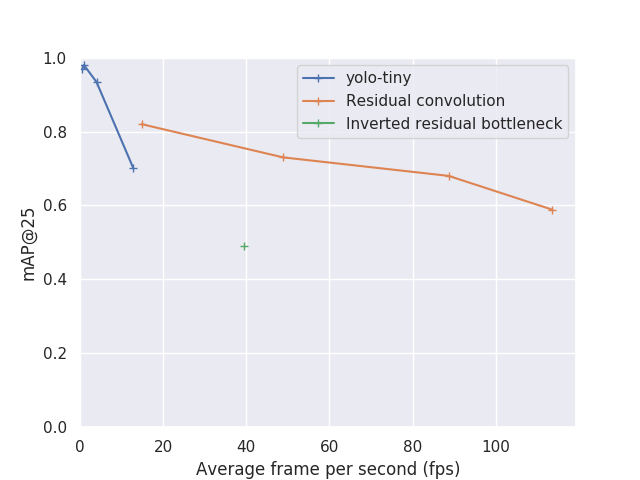
\includegraphics[width=0.99\linewidth]{figures/map_at_25_fps_models.png}
      \caption{Evolution of the mAP@25 with the frame per second}
    \end{subfigure}
    \caption{Plots of the ratio computation speed vs accuracy for different architectures, the residual block studied here and Yolov3-tiny, converted to TensorFlow lite with the code from \cite{benjamintanweihao2018Oct}. Speed are computed for a run on a Samsung S6 (SM-920T) using one thread.}
    \label{fig:map_to_speed}
  \end{center}
\end{figure}

\begin{table}[]
    \centering
    \caption{Value of the mAP, latency and frame per second for different configuration and different models. Numerical values used for the graphical representation of Figure \ref{fig:map_to_speed}}
    \begin{tabular}{|c|c|c|c|c|c|d{1}|}
        \hline
        Architecture & Input size & Filters & mAP@50 & mAP@25 & Latency (s) & \mathrm{FPS} \\ \hline
        \multirow{ 4 }{*}{ Yolov3-tiny } & 704x416 & - & 0.92 & 0.97 & 1.738 & 0.6 \\
    	  & 576x320 & - & 0.96 & 0.98 & 1.075 & 0.9 \\
    	  & 160x288 & - & 0.77 & 0.93 & 0.252 & 4.0 \\
    	  & 96x160  & - & 0.39 & 0.70 & 0.078 & 12.8 \\
    	\hline
    	\multirow{ 4 }{*}{ \shortstack{Residual\\convolution} } & 110x200 & (6,10) & 0.48 & 0.59 & 0.009 & 113.7 \\
    	  & 110x200 & (8,16) & 0.55 & 0.68 & 0.011 & 88.7 \\
    	  & 110x200 & (16,24) & 0.61 & 0.73 & 0.020 & 48.9 \\
    	  & 110x200 & (32,64) & 0.67 & 0.82 & 0.068 & 14.8 \\
    	\hline
    	Inverted & & & & & & \\
    	residual & 110x200 & (8,16) & 0.38 & 0.49 & 0.025 & 39.4 \\
    	bottleneck & & & & & & \\
    	\hline
    \end{tabular}
    \label{tab:map_to_speed}
\end{table}{}

Figure \ref{fig:map_to_speed} and Table \ref{tab:map_to_speed} show the evolution of the prediction speed on a mobile device and how the accuracy evolve with it. We also added values for Yolo v3 in its tiny version, as a comparison. The mAP value used in these graphs are the one get from the best training over all the combination we tried. The first thing to notice from this Figure, is the behavior of the inverted residual bottleneck. Speed is not even on the side of this block structure, that in addition to perform poorly is slower than is counterpart with the same amount of filters. Yolo, on another hand perform quite well on this task even on low resolutions. With an input size of $160\times288$ it reach a speed of $4fps$ while maintaining an mAP@50 of $77\%$. This speed is still too slow to be considered real time on a smartphone, but considering the accuracy it is still quite a good performance. But Yolo fail to reach higher speed as it is limited by its deep architecture. As you can see on Figure \ref{fig:map_to_speed}, its accuracy drop when trying to reach speed of $13fps$, with an input resolution of $96\times160$. Our architecture, with the residual convolution block and different filter size never manage to do better than $70\%$ of mAP@50 and has trouble to reach $80\%$ of mAP@25. However, as you will see on section \ref{sec:test}, this lower mAP is not really significant in real live use case. On the other side, our architecture, is able to maintain a good accuracy while decreasing the latency to extremely low level, allowing to run image object detection on a single thread of a smartphone faster than most camera are able to collect the images, leaving plenty of resource available to run other task simultaneously or simply saving energy and allowing longer battery live. Our fastest accurate model achieve $55\%$ mAP@50 and $68\%$ mAP@25 while running at $88fps$ on our test smartphone, a four years old model. The gap between mAP@50 and mAP@25 show that our model is however not very accurate in the localization of the object, but that was one of our core starting assumptions in Chapter \ref{chapter:technicalApproach} Section \ref{Assumptions}.

If our model manage to get good results, these results are evaluated according to a single metric, even if this metric is the reference in object detection filed, it is not perfect. In addition, if the validation data used to compute these values are never seen during training by the model, they came from the same set of data and so may have the same diversity, missing the same complex cases. It is so very important to conduce a more complete set of testing, in order to get a validation of the results we get previously.

\section{Testing results} \label{sec:test}
\subsection{Introduction}
\paragraph{}
In this section we are going to present the results of test we conduced on different set of data. This data were not annotated, preventing us to produce numbering such as mAP or any other metric. Our goal here is so more to represent how our model is performing in the wild, on real use cases. We are so going to present example of detection on different kind of road, with different traffic sign quality.

In this section we are going to review the results of one model. We chose here to evaluate the model based on residual convolution and with filters $(8,16)$, as it provide a very high processing speed, reaching $88fps$, while maintaining a good accuracy as you can see on Table \ref{tab:map_to_speed}. Our goal here is to illustrate what a low mAP mean on this model.

Because this section is a test, it is important to stress that our training data does not have any images took on these roads, and so they appear completely new to our algorithm. Also, as it is a final test, we did not to tune our model to improve the results, this is the final results after defining our model on the training and validation set. Some tuning will definitely improve the results, but will make it less close to a real use case we are simulating here.

\subsection{State Road 2} \label{sec:sr2}
\subsubsection{Presentation}
\paragraph{}
State road 2, in Georgia is one of the main testing site of our team. Figure \ref{fig:map_sr2} show the map of the section used for testing. This section of 21km (13 miles), have been chosen for it is high density of curve, resulting in a high density of warning sign in the area.

\begin{figure}
    \centering
    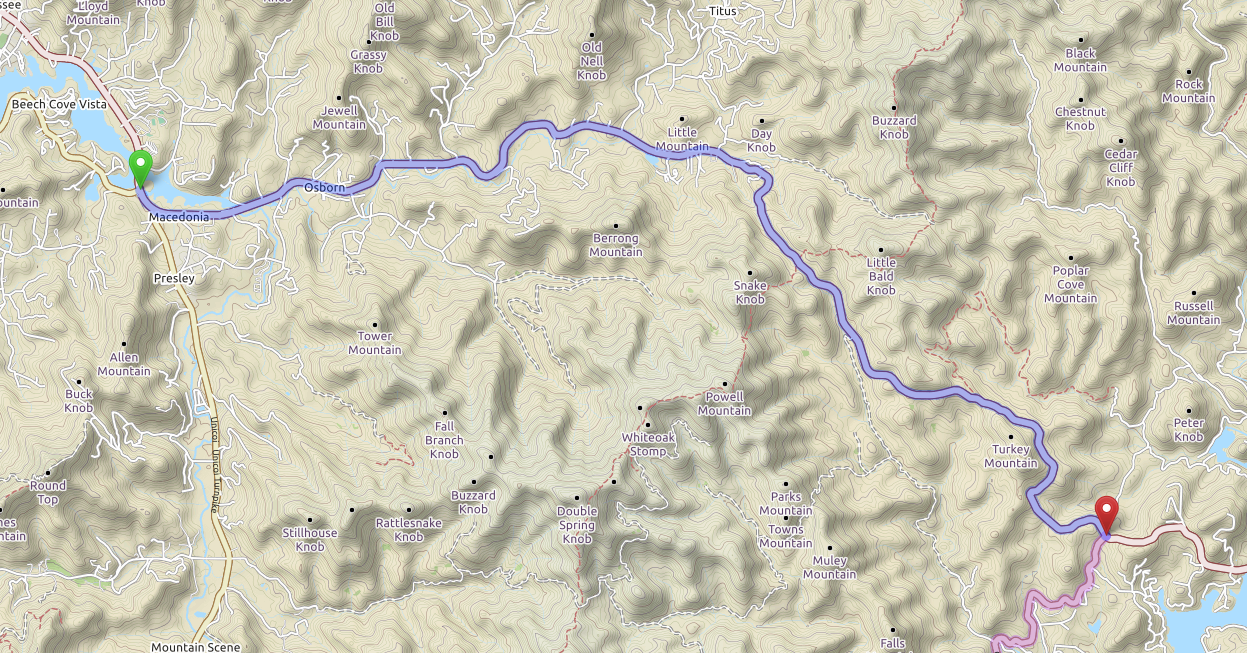
\includegraphics[width=0.8\linewidth]{figures/map_sr2.png}
    \caption{Map representing the test section we used on State Road 2}
    \label{fig:map_sr2}
\end{figure}{}

Being a state road, this area receive more care from the Department Of Transportation (DOT) than other areas, resulting on signs that are in better condition and are generally not obstructed by trees. In total there is more than one hundred signs on this section. From all the $70,438$ on which the model was run, and we reviewed we collected some interesting examples for each category that we are going to display bellow.

\subsubsection{False Positive cases}

\begin{figure}
  \begin{center}
    \begin{subfigure}[t]{.49\linewidth}
      \centering
      
\includegraphics[width=0.99\linewidth]{figures/examples/sr2/FP/FP_13.png}
      \caption{Chevron Sign}
      \label{fig:chevronFP}
    \end{subfigure}
    \begin{subfigure}[t]{.49\linewidth}
      \centering
      
\includegraphics[width=0.99\linewidth]{figures/examples/sr2/FP/FP_09.png}
      \caption{Guard rail signalization}
      \label{fig:guardRailFP}
    \end{subfigure}
    \begin{subfigure}[t]{.49\linewidth}
      \centering
      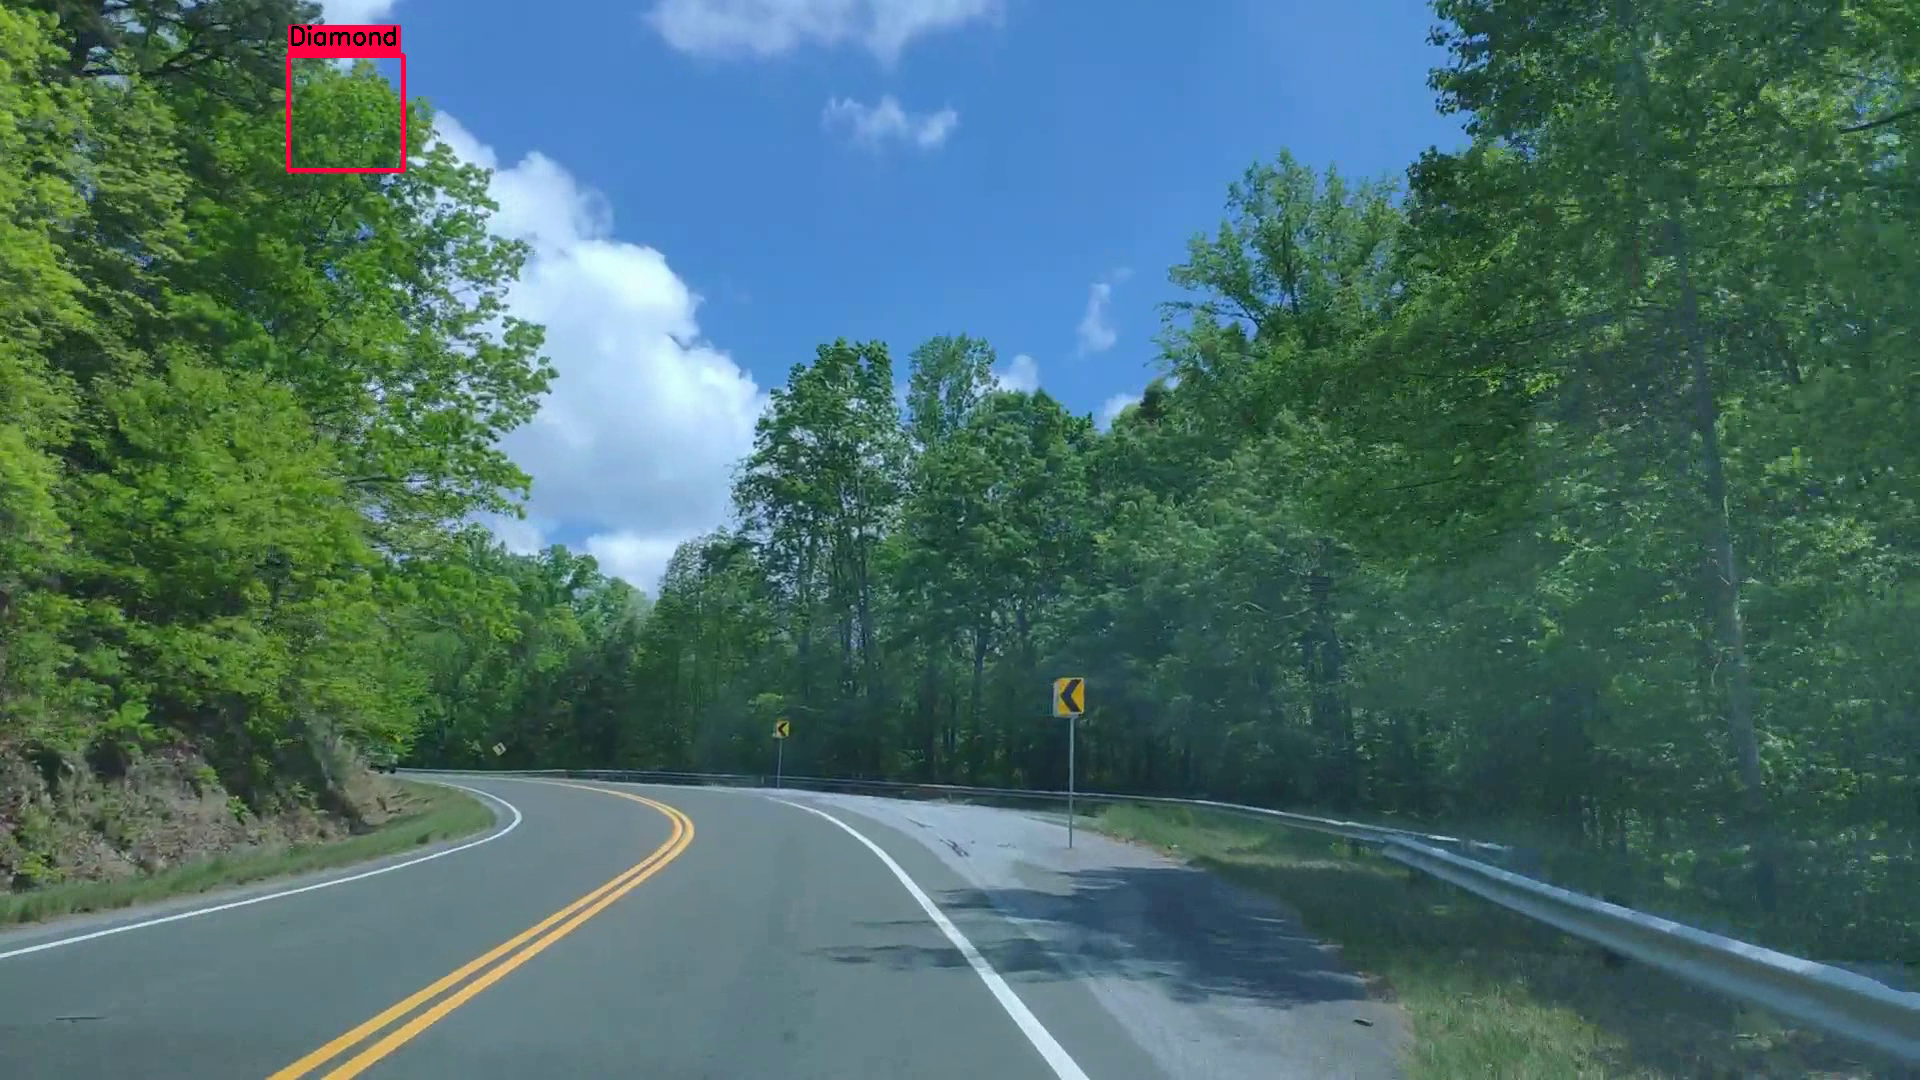
\includegraphics[width=0.99\linewidth]{figures/examples/sr2/FP/FP_04.png}
      \caption{Plants}
      \label{fig:plantFP}
    \end{subfigure}
    \begin{subfigure}[t]{.49\linewidth}
      \centering
      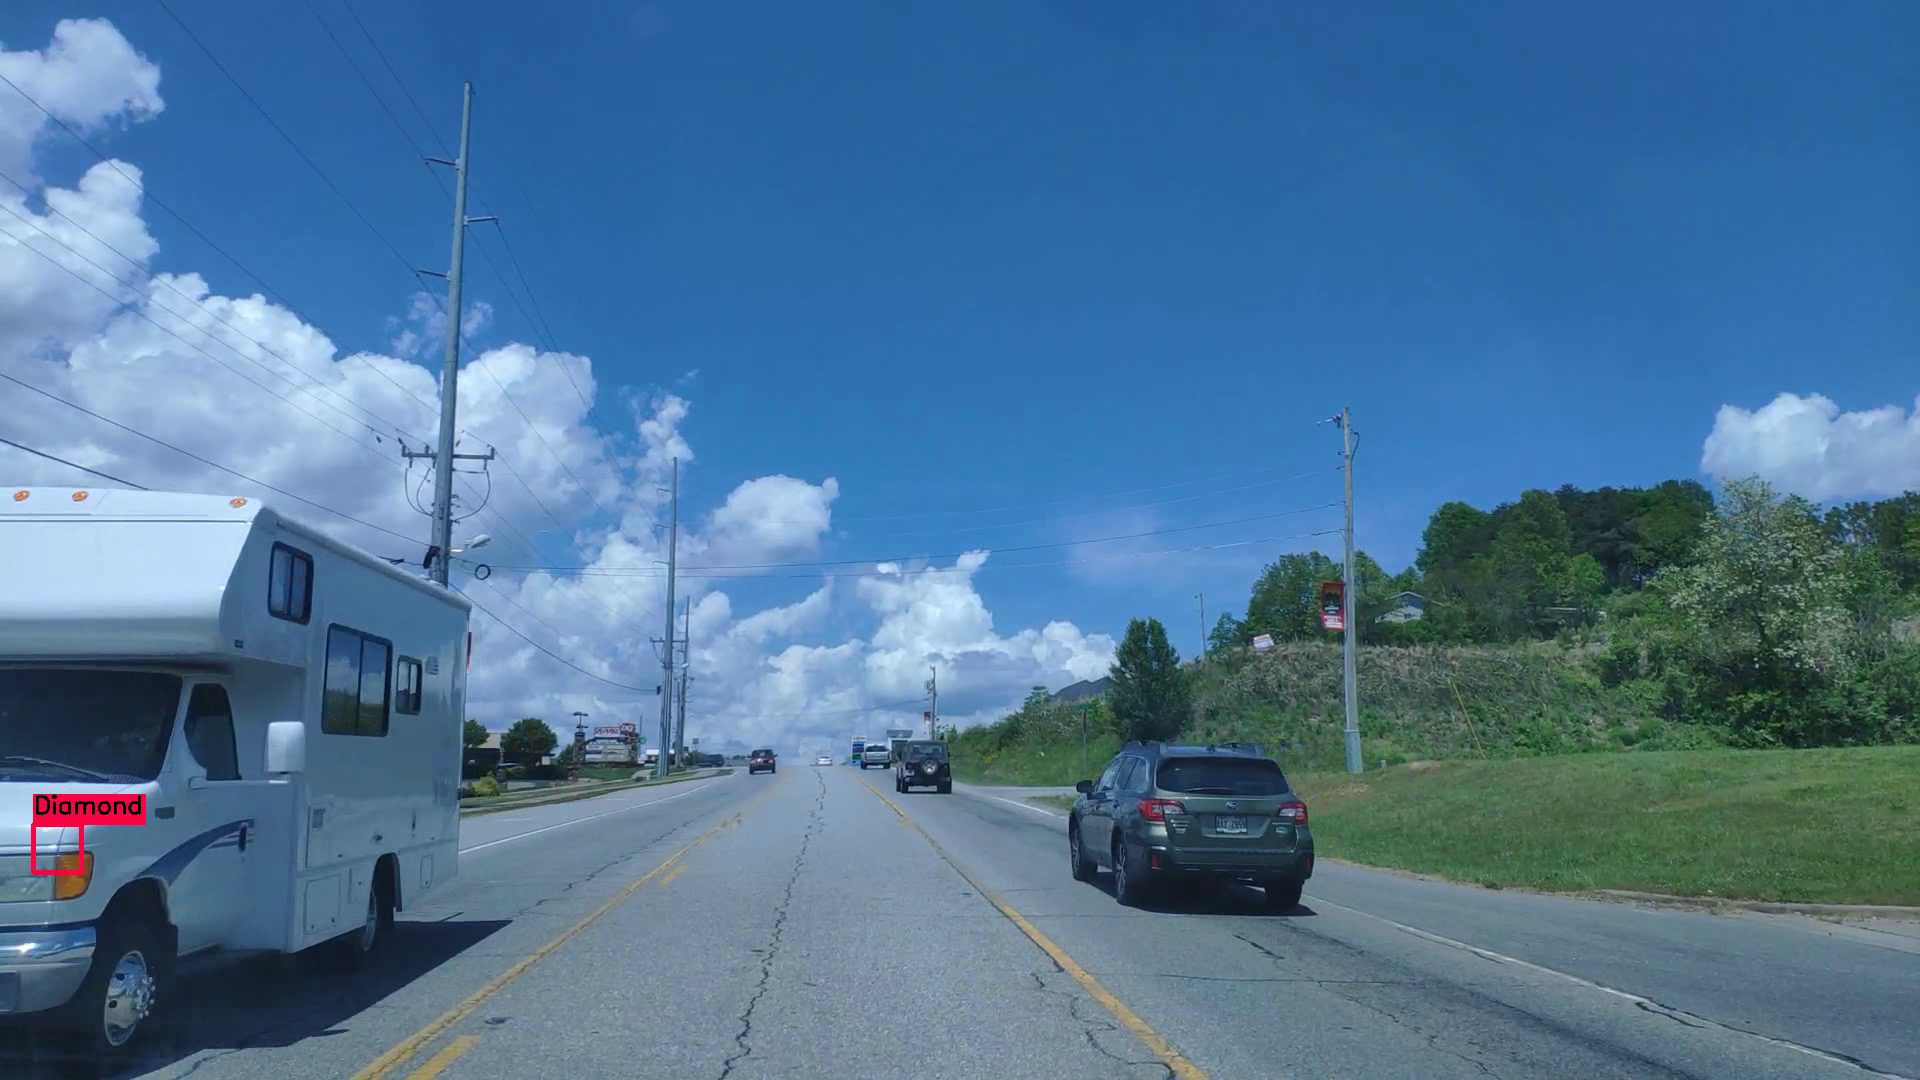
\includegraphics[width=0.99\linewidth]{figures/examples/sr2/FP/FP_19.png}
      \caption{Car Light}
      \label{fig:carLightFP}
    \end{subfigure}
    \begin{subfigure}[t]{.49\linewidth}
      \centering
      
\includegraphics[width=0.99\linewidth]{figures/examples/sr2/FP/FP_01.png}
      \caption{Yellow signalization}
      \label{fig:GDOTtruckFP}
    \end{subfigure}
    \begin{subfigure}[t]{.49\linewidth}
      \centering
      
\includegraphics[width=0.99\linewidth]{figures/examples/sr2/FP/FP_03.png}
      \caption{Yellow digger}
      \label{fig:diggerFP}
    \end{subfigure}
    \begin{subfigure}[t]{.49\linewidth}
      \centering
      
\includegraphics[width=0.99\linewidth]{figures/examples/sr2/FP/FP_07.png}
      \caption{Work zone diamond sign}
      \label{fig:workzoneFP}
    \end{subfigure}
    \begin{subfigure}[t]{.49\linewidth}
      \centering
      
\includegraphics[width=0.99\linewidth]{figures/examples/sr2/FP/FP_17.png}
      \caption{Advertisement sign}
      \label{fig:advertisementFP}
    \end{subfigure}
    \caption{Example of False Positive case collected on State Road 2.}
    \label{fig:FPcases}
  \end{center}
\end{figure}

\paragraph{}
Our model as tendency to detect some yellow object as diamond traffic signs. In most of the cases, this false positive (FP) detection happen on other warning signs that are not supposed to be detected by this model and so were not part of the training data. This is the case illustrated by Figure \ref{fig:chevronFP}, this case is by far the most important case of FP, with more than twenty of them. However, this case is not really problematic because it is a sign, the best approach to fix this is to include it into the training as a new class. Another case of sign that are miss detected is the work zone sign, as illustrated by figure \ref{fig:workzoneFP}, we encountered six different signs like that in our testing, here the best solution to counter that is to wait a classification step to correct it. It is important to notice that most of the work zone signs are not detected as expected.

Another category of false positive we observed, is the yellow signalization. A first example is the signalization at the beginning of a guard rail. This case is illustrated on Figure \ref{fig:guardRailFP}, we observed three such case on the entire run. The second one is the signalization on the back of the Georgia DOT truck we were following the whole time. We get two FP out of this warning bend as illustrated on Figure \ref{fig:GDOTtruckFP}.

The remaining FP were yellow object present around the road. This kind of objects include, a car light from Figure \ref{fig:carLightFP}, a part of a yellow digger, on Figure \ref{fig:diggerFP}, yellow advertisement signs as in Figure \ref{fig:advertisementFP} or plants like displayed on Figure \ref{fig:plantFP}. Of all those case, only the last two appeared three times while the other only once on all the frames, and they all appear only in one frame, making them easy to filter out.

All this example show more a weakness of the dataset we use for training than a real failure our architecture, although, the final number of false positive we get were is still small regarding the number of true positive.

\subsubsection{False Negative cases}

\begin{figure}
  \begin{center}
    \begin{subfigure}[t]{.49\linewidth}
      \centering
      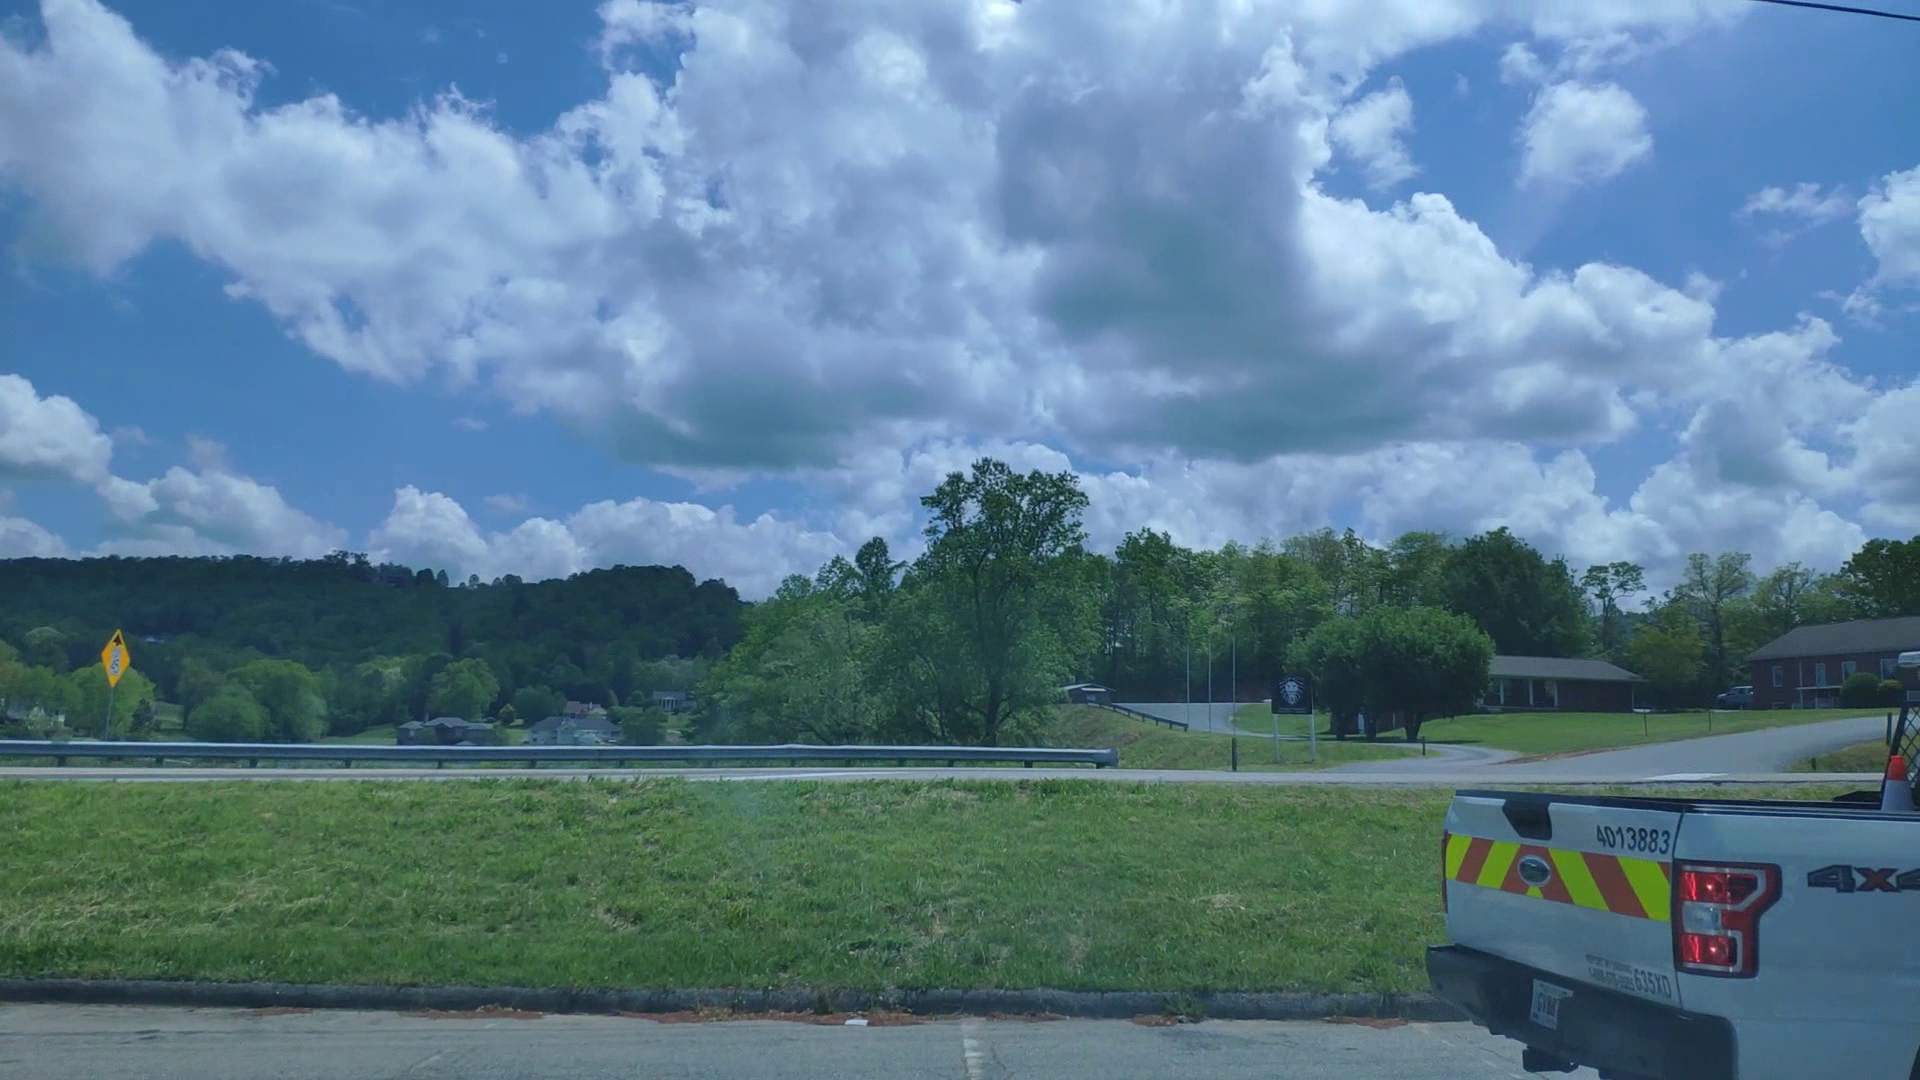
\includegraphics[width=0.99\linewidth]{figures/examples/sr2/FN/FN_01.png}
      \caption{Perspective transformation}
      \label{fig:perspecFN}
    \end{subfigure}
    \begin{subfigure}[t]{.49\linewidth}
      \centering
      
\includegraphics[width=0.99\linewidth]{figures/examples/sr2/FN/FN_02.png}
      \caption{Light, faded sign}
    \end{subfigure}
    \begin{subfigure}[t]{.49\linewidth}
      \centering
      
\includegraphics[width=0.99\linewidth]{figures/examples/sr2/FN/FN_03.png}
      \caption{Light, faded sign}
    \end{subfigure}
    \begin{subfigure}[t]{.49\linewidth}
      \centering
      
\includegraphics[width=0.99\linewidth]{figures/examples/sr2/FN/FN_09.png}
      \caption{Sign on the other side of the road}
      \label{fig:othersideFN}
    \end{subfigure}
    \begin{subfigure}[t]{.49\linewidth}
      \centering
      
\includegraphics[width=0.99\linewidth]{figures/examples/sr2/FN/FN_10.png}
      \caption{Light, faded sign}
    \end{subfigure}
    \begin{subfigure}[t]{.49\linewidth}
      \centering
      
\includegraphics[width=0.99\linewidth]{figures/examples/sr2/FN/FN_06.png}
      \caption{Light, faded sign}
    \end{subfigure}
    \begin{subfigure}[t]{.49\linewidth}
      \centering
      
\includegraphics[width=0.99\linewidth]{figures/examples/sr2/FN/FN_07.png}
      \caption{Light, faded sign}
    \end{subfigure}
    \begin{subfigure}[t]{.49\linewidth}
      \centering
      
\includegraphics[width=0.99\linewidth]{figures/examples/sr2/FN/FN_08.png}
      \caption{Light, faded sign}
    \end{subfigure}
    \caption{Example of False Negative cases collected on State Road 2.}
    \label{fig:FNcases}
  \end{center}
\end{figure}

\paragraph{}
In total, we counted 10 FN on this set of frames. One in Figure \ref{fig:perspecFN}, is due to a large perspective transformation and a small size. We can note that this sign is latter detected when driving on the road. Another case, representing two false positive, is sign on the left side of the road, one of these cases is illustrated by Figure \ref{fig:othersideFN}, such cases are more difficult to detect because of the orientation of the camera and in both of these cases poor lighting condition and sign condition. However, the most common case is light, faded sign that are not properly detected, as you can see on Figure \ref{fig:FNcases}. This number of similar case, let us believe that it is a result of the lack of diversity in our training data. One way to fix that would be to set up a more aggressive data augmentation on the color point of view. More experiments are needed to rule about the responsibility of the model.

\subsubsection{Interesting True positive cases}

\begin{figure}
  \begin{center}
    \begin{subfigure}[t]{.49\linewidth}
      \centering
      \includegraphics[width=0.99\linewidth]{figures/examples/sr2/TP/TP_01.png}
      \caption{Temporary sign}
      \label{fig:temporaryTP}
    \end{subfigure}
    \begin{subfigure}[t]{.49\linewidth}
      \centering
      \includegraphics[width=0.99\linewidth]{figures/examples/sr2/TP/TP_09.png}
      \caption{Small and partially obstructed sign}
      \label{fig:farobstTP}
    \end{subfigure}
    \begin{subfigure}[t]{.49\linewidth}
      \centering
      \includegraphics[width=0.99\linewidth]{figures/examples/sr2/TP/TP_05.png}
      \caption{Multiple signs in different conditions}
      \label{fig:multipleTP}
    \end{subfigure}
    \begin{subfigure}[t]{.49\linewidth}
      \centering
      \includegraphics[width=0.99\linewidth]{figures/examples/sr2/TP/TP_08.png}
      \caption{Small sign}
      \label{fig:smallTP}
    \end{subfigure}
    \begin{subfigure}[t]{.49\linewidth}
      \centering
      \includegraphics[width=0.99\linewidth]{figures/examples/sr2/TP/TP_02.png}
      \caption{Temporary sign of different size}
      \label{fig:bigtempTP}
    \end{subfigure}
    \begin{subfigure}[t]{.49\linewidth}
      \centering
      \includegraphics[width=0.99\linewidth]{figures/examples/sr2/TP/TP_04.png}
      \caption{Obstructed Sign}
      \label{fig:obstTP}
    \end{subfigure}
    \caption{Example of True positive cases collected on State Road 2.}
    \label{fig:TPcases}
  \end{center}
\end{figure}

\paragraph{}
Given the simplicity and the input size of our model, during our review, we were pleased to note different cases of True Positive (TP). One of them are the temporary warning signs displayed on Figure \ref{fig:temporaryTP} and \ref{fig:bigtempTP}, these signs are not part of our training data and are slightly different from the sign usually on the road, we were so pleased to see the model generalize on that point. Given the size of the input and the smallest possible anchors, $3\times3$, we were not expecting much detection at this size, but our experiment proved us wrong with lot of small sign being accurately detected, as you can see on Figure \ref{fig:smallTP}. Another difficult case that is not well represented on our dataset is the obstructed case. We did not do anything to help the network understand that sign could be hidden, but the model still manage to detect them properly, as you can see on Figure \ref{fig:obstTP} or also on Figure \ref{fig:farobstTP}, where the signs are barely visible on the full resolution image.

\subsection{West Westley}
\subsubsection{Presentation}
\paragraph{}
West Westley is another usually test site for our team, located in the residential area near Atlanta, it has been chosen because of the easy access it provides and its small curvy road with lot of vegetation around, making the signs sometimes difficult to detect. If this road is a usual test bed for our team, our training data does not include any of these roads.

\begin{figure}
    \centering
    \includegraphics[width=0.8\linewidth]{figures/westwestleymap.png}
    \caption{Map representation of the West Westley test road.}
    \label{fig:wwmap}
\end{figure}{}

This test section is a 9km (5.6 Miles) long road in a residential area. As you can see on Figure \ref{fig:wwmap}, this road goes into lot of curves in high population area, but out of main large roads. The video collected is composed of $22,198$ frames, on witch we counted $34$ diamond warning signs. After reviewing the 12 minutes long video we got $10$ false positive cases (FP), $3$ false negative (FN) and $31$ true positive (TP). These numbers are also given on table \ref{tab:ww_numbers}, were you can see that our final precision is over two third, meaning that over two third of the object detected are actual diamond warning sign, this number goes even higher if you think in term of frames, as FP detection are generally limited to less than three frames. In term of recall, we get over the $90\%$ threshold, meaning that most of the signs are detected, and as we will see in the following, the missed signs represented difficult cases.

\begin{table}[]
    \centering
    \caption{Quantitative results for the test on West Westley. The numbers are given based on individual signs or object detected not on frame with detection.}
    \begin{tabular}{|c|c|c|c|c|c|c|}
        \hline
        Frame count & Sign count & TP & FP & FN & Precision & Recall \\ \hline
        $22,198$ & $34$ & $31$ & $10$ & $3$ & $76\%$ & $91\%$ \\ \hline
    \end{tabular}
    \label{tab:ww_numbers}
\end{table}{}

In the following we are going to give more detail about what is the reality behind these numbers, illustrating how our model behave in real application in this kind of context.

\subsubsection{False Positive cases}
\begin{figure}
  \begin{center}
    \begin{subfigure}[t]{.49\linewidth}
      \centering
      \includegraphics[width=0.99\linewidth]{figures/examples/westwestley/FP/FP01.jpg}
      \caption{Chevron sign}
      \label{fig:wwChevronFP}
    \end{subfigure}
    \begin{subfigure}[t]{.49\linewidth}
      \centering
      \includegraphics[width=0.99\linewidth]{figures/examples/westwestley/FP/FP02.jpg}
      \caption{Small yellow flag}
      \label{fig:wwFlag1FP}
    \end{subfigure}
    \begin{subfigure}[t]{.49\linewidth}
      \centering
      \includegraphics[width=0.99\linewidth]{figures/examples/westwestley/FN/FN01.jpg}
      \caption{Speed limit}
      \label{fig:wwslFP}
    \end{subfigure}
    \begin{subfigure}[t]{.49\linewidth}
      \centering
      \includegraphics[width=0.99\linewidth]{figures/examples/westwestley/FP/FP05.jpg}
      \caption{School Sign (MUTCD: S1-1)}
      \label{fig:wwSchoolFP}
    \end{subfigure}
    \begin{subfigure}[t]{.49\linewidth}
      \centering
      \includegraphics[width=0.99\linewidth]{figures/examples/westwestley/FP/FP06.jpg}
      \caption{Back of traffic light}
      \label{fig:wwTraffficLight1FP}
    \end{subfigure}
    \begin{subfigure}[t]{.49\linewidth}
      \centering
      \includegraphics[width=0.99\linewidth]{figures/examples/westwestley/FP/FP07.jpg}
      \caption{Chevron sign}
      \label{fig:wwChevron2FP}
    \end{subfigure}
    \begin{subfigure}[t]{.49\linewidth}
      \centering
      \includegraphics[width=0.99\linewidth]{figures/examples/westwestley/FP/FP08.png}
      \caption{Temporary sign}
      \label{fig:wwTemporaryTP}
    \end{subfigure}
    \begin{subfigure}[t]{.49\linewidth}
      \centering
      \includegraphics[width=0.99\linewidth]{figures/examples/westwestley/FP/FP09.png}
       \caption{Back of traffic light}
      \label{fig:wwTraffficLight2FP}
    \end{subfigure}
    \caption{Example of false positive cases collected on West Westley.}
    \label{fig:wwFPcases}
  \end{center}
\end{figure}

\paragraph{}
Of the $10$ FP detection on this test, $5$ are actual traffic signs and $1$ is a temporary traffic sign. The most common case of sign being detected is, as in Section \ref{sec:sr2} about state road 2, chevron signs. Example of such detection are given on Figure \ref{fig:wwChevronFP} and \ref{fig:wwChevron2FP}. Another sign that was mistaken as a diamond warning sign is the school warning sign, as displayed on Figure \ref{fig:wwSchoolFP}. This sign is special as it has an irregular pentagon shape with the top half looking exactly as a diamond sign. We also get the interesting case of a warning speed limit being detected, while the actual sign above it is not, this case is displayed on Figure \ref{fig:wwslFP}. The last case of sign that was miss detected is the temporary board displayed on Figure \ref{fig:wwTemporaryTP}.

The remaining false positive consist of the yellow back of traffic light as illustrated by Figure \ref{fig:wwTraffficLight1FP} and \ref{fig:wwTraffficLight2FP} and of small yellow construction flag on the side of the road, which you can see on Figure \ref{fig:wwFlag1FP}.

All this exact false positive cases were also encountered in other models trained over the same training data, this model, namely Yolov3-spp, is much more complex than our currant model, the fact that it still produce the same mistake raise large question about the coverage of the dataset we use. We were even surprised that our model detect them less frequently than the Yolov3-spp model, this is probably due to the smaller complexity of our model forcing it to generalize more. All this False Positive cases are only detected on less than five frames showing that adding a few more example during training could improve the results a lot.

\subsubsection{False Negative cases}
\paragraph{}
This test section revealed three different case of false positive. The first one, displayed on Figure \ref{fig:wwWhiteFN}, was already encountered in Section \ref{sec:sr2}, it consists of a whitened and faded sign with not very bright yellow color. The case of Figure \ref{fig:wwFaddedFN} is even more difficult, the sign is covered by a green algae and under the shadow of a pine tree making it particularly difficult to detect. Finally, the last case of False Negative detection happen on the ramp to exit the high way, it consists of a sign on the edge of the video, often obstructed by the sign in front of it. In addition, this sign that you can see on Figure \ref{fig:wwobsFN}, is whiter than usual, a case that our model as trouble to detect.
\begin{figure}
  \begin{center}
    \begin{subfigure}[t]{.49\linewidth}
      \centering
      \includegraphics[width=0.99\linewidth]{figures/examples/westwestley/FN/FN01.jpg}
      \caption{Whitened sign}
      \label{fig:wwWhiteFN}
    \end{subfigure}
    \begin{subfigure}[t]{.49\linewidth}
      \centering
      \includegraphics[width=0.99\linewidth]{figures/examples/westwestley/FN/FN02.jpg}
      \caption{Dirty, faded sign in the shadow}
      \label{fig:wwFaddedFN}
    \end{subfigure}
    \begin{subfigure}[t]{.49\linewidth}
      \centering
      \includegraphics[width=0.99\linewidth]{figures/examples/westwestley/FN/FN03.png}
     \caption{Small often obstructed sign}
      \label{fig:wwobsFN}
    \end{subfigure}
    \caption{Example of false negative cases collected on West Westley.}
    \label{fig:wwFNcases}
  \end{center}
\end{figure}


\subsubsection{Interesting True Positive cases}
\paragraph{}
Considering the simplicity of our model and the input resolution, we were pleased to see that we were able to manage all the cases where the signs were obstructed by trees on this road. Figure \ref{fig:wwTPcases} show some example of such successful detection in non-trivial cases.

\begin{figure}
  \begin{center}
    \begin{subfigure}[t]{.49\linewidth}
      \centering
      \includegraphics[width=0.99\linewidth]{figures/examples/westwestley/TP/TP04.jpg}
      \caption{Obstructed sign}
      \label{fig:wwObs1TP}
    \end{subfigure}
    \begin{subfigure}[t]{.49\linewidth}
      \centering
      \includegraphics[width=0.99\linewidth]{figures/examples/westwestley/TP/TP02.jpg}
      \caption{Obstructed sign}
      \label{fig:wwObs2TP}
    \end{subfigure}
    \begin{subfigure}[t]{.49\linewidth}
      \centering
      \includegraphics[width=0.99\linewidth]{figures/examples/westwestley/TP/TP05.png}
      \caption{Obstructed sign}
      \label{fig:wwObs3TP}
    \end{subfigure}
    \caption{Example of true positive cases collected on West Westley.}
    \label{fig:wwTPcases}
  \end{center}
\end{figure}

\subsection{Conclusion}
\paragraph{}
In this section we demonstrated the generalization of our results on the validation data to real use cases. Showing that, if the accuracy of our model does not reach state-of-the-art object detection levels, it does achieve very good results, that can be used on real live while speeding up the detection process by a one hundred factor allowing to be run directly on a smartphone.

\section{About localization}
\paragraph{}
You probably noticed on all the images examples given previously, that most of the time the detection box is off the sign and is not perfectly at the right size. There is even cases like on Figure \ref{fig:multipleTP} where the box is completely outside the sign. To interpret this results, it is important to remember the assumption from Chapter \ref{chapter:technicalApproach} Section \ref{Assumptions}. Our model is not trying to draw a perfect box around an object, but is instead trying to give the approximate position and approximate size of the object to detect. 

In most of the application this approximated position and size are enough to get what you need, especially in a traffic sign detection context where getting pixel accurate box around the sign does not add lot of value. Even if this accuracy is not enough for a given task, the computation speed to get this results is so fast that you that you can use a post processing that will refine the box locally and still be faster than other larger models because you will skip most of the useless frames.

\section{Conclusion}
\paragraph{}
In this chapter we used the tools defined in Chapter \ref{chapter:technicalApproach} to build an efficient architecture, exploring its behavior over our dataset. We trained it over our artificial dataset and showed the improvement it brings to the final results. We finally studied the results of our model in term of computation efficiency, comparing it to well known architecture, and concluded by testing the resulting model on real live application, to exhibit the strange and weakness of our approach, showing that this approach successfully solve our problem and is ready for real life usage. However, improvement can still be made and lot of open research question are still unsolved, calling for additional research on that field.





%%%%%%%%%%%%%%%%
% Chapter 4
%%%%%%%%%%%%%%%%

\chapter{Discussion}

\paragraph{}
This study showed that detecting traffic sign on low end devices mobile is now possible. However, there is still a wide range of possible improvement and experimentation to explore, this research also open the way to a wide range of application ranging from infrastructure assessment to real time driver assistance and autonomous driving.

\paragraph{}
The scope of this study was limited to the detection of US warning signs. During this study we trained and tested our model on a wide range of cases, with data collected from Georgia and other neighboring states. More testing would allow to get a better assessment of the performance of the model. One example of case the model never encountered is snow. While show is not impossible in that region of the United States, it is fairly uncommon and does not appear on our data. So doing additional testing would allow a better assessment of the quality of the model.

The model was designed with multiple class detection in mind, but this functionality was never tested because out of the scope of this work. Using multiple class detection could, however, improve the detection by improving the feature extracted by the backbone network. On an application point of view, this will also allow to have a larger impact. We advise in this case to define different anchors for each classes, while trying to stay at similar scales.

This study was also focused on the creation of an architecture that is able to run on mobile devise. If we have some demo and test demonstrating these capabilities, they are packaged for production. A future task could be to implement a proper pipeline in mobile device to run the detection, as well as other processing step, such as classification, directly on the device. This would allow a production usage of the method developed here.

We tested and tuned our model to run on a Samsung S6 (SM-G920T), this device is not completely outdated, but is still far from the performance of newer smartphone. This was done on purpose, you do not want the model to only run on recent flagship devices, but also to run a nearly any smartphone available on the market. However, taking advantage of the newer devices should allow producing deeper and better models. This area is not explored here and is left open to latter research.

A classical approach to speed up inference on mobile device is to use model quantification. We described this approach in Chapter \ref{subsec:optMobileDevice}. During our experiment we used weights quantification, which speed up the inference my a small amount, but is mainly designed to reduce the size of the weights to transfers to the mobile device. We planned to use full model quantification, that have shown to give great results on mobile device, giving large speed-up while reducing the accuracy by only a small amount. Unfortunately, due to a bug in the current TensorFlow version (2.0.0) we were not able to explore this solution. Using this method should bring some more speed up and provide even better performances. Latter research should be able to use that to provide a large improvement over the current results.

Lot of previous study \cite{sandler2018mobilenetv2, howard2019mobilenetv3} showed the benefit of using architecture such as Inverted residual bottleneck on mobile device. During this study we were not able to reproduce such benefit. During our experiment the inverted residual bottleneck were at best as accurate as a residual convolution but slower on a mobile device. The true benefit of this kind of block may only come after a complete quantification of the network, which we were not able to perform as stated previously. In \cite{howard2019mobilenetv3} the authors proposed to add an attention mechanism improving the results a bit more, as well as the switch activation function on last layers. We did not try to implement those improvements because of the results we get on the original version, but ultimately this structure is supposed to improve the performance of the model and is so a good starting point for latter research.

As we discussed previously, we purposely reduced the localization and size accuracy of this model in order to make the task easier. However, it is still unclear how much speed up we were able to get from this reduced accuracy, testing similar architecture with added localization and size prediction may help to quantify the effect of these choices, and could improve the mAP results.

To improve accuracy, we also propose a way to artificially generate data for training. If we showed that this data helped a lot to improve the final results, we believe that a lot of things can be added to this procedure to make it more diverse and cover slightly more realistic case. Some of this improvement could be to add shadow like shape, add motion blur or simply use gradient in the shape instead of flat colors.

\paragraph{}
This work brings large improvement on the traffic sign detection on mobile device, but is only the starting point of this approach. If generic object detection is a problem that is globally solved, doing it with low computational impact is still an open problem. Here we fine-tuned an architecture for this particular task, but our research space did not cover all the possibilities which leave open questions for future research.




%%%%%%%%%%%%%%%%
% Chapter 5
%%%%%%%%%%%%%%%%

\chapter{Conclusion}

\paragraph{}
In this work we propose a new architecture to detect traffic signs in real time on mobile devices. This architecture is based on a new low localization accuracy head, allowing to simplify the task of object detection and making it possible to reduce the backend network to its core.

This proposed architecture reaches a prediction speed of 88fps on a smartphone (Samsung S6, SM-G920T), while maintaining a mAP@50 of 55\%, and a mAP@25 of 68\% on our data. While a mAP@50 over 95\% can be reached by model like Yolov3, such level of accuracy needs models that use much larger backend that allow them to run real time on big GPU, but is impossible to run on a mobile device.

To achieve these results we also propose a simple way to generate training data, using simple geometric shapes to help the network understand what is expected on the task and better utilize the real data.

\paragraph{}
To the best of our knowledge, this work improves the speed of traffic sign detection on a mobile device by more than a factor of 10 and opens the possibility of large range of mobile, real time applications.



%%%%%%%%%%%%%%%%
% Appendices
%%%%%%%%%%%%%%%%

\begin{appendices}

%Some Table of Contents entry formatting
\addtocontents{toc}{\protect\renewcommand{\protect\cftchappresnum}{\appendixname\space}}
\addtocontents{toc}{\protect\renewcommand{\protect\cftchapnumwidth}{6em}}

%Begin individual appendices, separated as chapters

\chapter{Data} \label{data}
\section{Introduction}
\paragraph{}
During this study we relied for our experiments on a dataset collected and annotated in our team. In this appendix we are going to give more information about this data. From the way we got the base image to distribution of the data on this set, going by the annotation tool we used as the diversity of the case represented.

\section{Data collection}
\paragraph{}
This dataset consist of image of the road taken from the driver perspective with annotations of the visible signs. The data came from two different sources, the first one is image from Nashville DOT, collected by there survey vehicle, equipped with externally mounted high resolution camera. The large majority of the data was, however, collected by our team around Atlanta and in north Georgia. This data collection was done with smartphones and an application specially build for this purpose.

The smartphone used for data collection were of two different model, Xiaomi Redmi 4 and Xiaomi 8. Both of them recorded the video at full HD resolution, at 10 frame per second for the Redmi 4 and 30 frame per second for the Xiaomi 8. Aside from the frame rate, the image quality of this two devices is also completely different. The Redmi 4 produce image that are more blurry and sensitive to over and under exposure, leading to a much lower image quality than Xiaomi 8 that produce much sharper images, although with less natural color that tend to be more blueish.

The Android application we used to collect the data was developed internally and named AllGather. During the data collection the smartphone was attached to the windshield, as displayed on Figure \ref{fig:windshield}. In this setting the smartphone collect the video, as well as the GPS, the acceleration and the value from the magnetometer. Once the the recording the started, it's only needed to drive around the road to collect the data.

\begin{figure}
    \centering
    \includegraphics[width=0.5\linewidth]{figures/smartphone-datacolection.jpg}
    \caption{Example of the setup used for data collection}
    \label{fig:windshield}
\end{figure}{}


This process allow to record realistic data real word data, as they are not collected by expensive camera in a especially designed setup. In particular, in addition to the image quality, our image have a fair amount of reflection from the windshield as well as dust. Making this dataset very close to the typical use case.


\section{Data annotation}
\paragraph{}
To perform this study, image alone were not valuable, the more important things is the annotation. To ensure the highest accuracy possible, our team annotated the data internally using a especially made software. 

The software we used for this task is an internal tool developed in C\# to take into account the specificity of our task, especially the video aspect of it. This tool was made to provide more than just the position and class of the signs, it also allow to give id to the signs and signpost or poll. It also implement pattern matching algorithm to make the process of annotating data easier.

This tool was used to annotate all the $652,321$ frames collected, counting $8,719$ sign images spitted in $39$ different classes.

\section{Label distribution}
\paragraph{}
Because our dataset represent the distribution of signs on the local roads of north Georgia. The distribution of the labels in our dataset is quite unbalanced. As you can see on Figure \ref{fig:data_count} and Table \ref{tab:data_count}, some classes of signs are much more represented than other. However, as we only care about detection and not classification, we can group all the warning signs together summing to $8,348$ signs that can be used for training detection. Allowing us to use $8,719$ images during the experiments presented in this document.

\begin{figure}
    \centering
    \includegraphics[width=\linewidth]{figures/data_repartition.png}
    \caption{Count of example for each classes in the dataset, cropped to 250 for readability.}
    \label{fig:data_count}
\end{figure}{}

\begin{table}[]
    \centering
    \begin{tabular}{|l|r|}
    \hline
        \textbf{Sign class} & \textbf{Count} \\ \hline
        W1-1a\_15\_L & 1\\
        W1-1\_L & 56\\
        W1-1\_R & 21\\
        W1-2\_L & 1365\\
        W1-2\_R & 1183\\
        W1-3\_L & 31\\
        W1-3\_R & 6\\
        W1-4\_L & 205\\
        W1-4\_R & 93\\
        W1-5\_L & 216\\
        W1-5\_R & 135\\
        W1-6\_L & 13\\
        W1-6\_R & 10\\
        W1-7 & 102\\
        W1-10\_R & 27\\
        W2-1 & 90\\
        W2-2\_L & 1021\\
        W2-2\_R & 647\\
        W3-1 & 166\\
        W3-2 & 85\\
        W3-3 & 135\\
        W4-1 & 129\\
        W4-1\_L & 1\\
        W4-1\_R & 2\\
        W4-2 & 236\\
        W4-3 & 38\\
        W5-2 & 34\\
        W6-3 & 12\\
        W7-1 & 146\\
        W11-2 & 76\\
        W11-8 & 84\\
        W12-1 & 2\\
        W14-1 & 126\\
        W14-2 & 9\\
        W14-3 & 9\\
        W16-7P & 7\\
        WorkZone & 47\\
        W-unknown-diamond & 10\\
        \hline
    \end{tabular}
    \caption{Number of sample for each sign in the dataset}
    \label{tab:data_count}
\end{table}{}

\section{Weather conditions}
Diversity is a key for a machine learning dataset to be successful. By definition, diversity depend on a lot of factor, but in this case one of the important one is the weather. Weather is the main factor defining how far and how clearly you can see objects. Lot of dataset are biased on that point, data are mostly collected in clear sunny day. This dataset is not an exception.

Most of the data where collected while on trip to other fields test. Test that were performed outdoor on pavement and require to avoid rain, ruling out lot of cloudy day in Georgia. However if we don't have bad weather conditions, we our dataset cover still a large set of cases, sunset and darker hours of the day are for example well covered. An illustration of such an image is provided in Figure \ref{fig:blue_hour}.

\begin{figure}
    \centering
    \includegraphics[width=.7\linewidth]{figures/blue_hour_example.jpg}
    \caption{Example of image taken after sunset present in the dataset}
    \label{fig:blue_hour}
\end{figure}{}

This kind of example are very important in the task of traffic sign detection as the appearance of the sign can very a lot under this luminosity condition with the effect of cars lights. this different weather condition also put more importance on the quality of the sign. Newer sign tend to better reflect the light and so are much more visible than old faded one in low light condition, while in plain day light this difference is not that important.

\section{Conclusion}
\paragraph{}
This dataset collected and annotated manually by our team, is a corner stone of this project. This dataset has it's own issue and could be improved, some weather conditions are missing, classes are largely unbalanced and the number of image is fairly limited. However, for our task of object detection on small scale models, such imperfection are not really critical.


\end{appendices}

%%%%%%%%%%%%%%%%
% References
%%%%%%%%%%%%%%%%

\begin{singlespace}  % use single-line spacing for multi-line text within a single reference
	\setlength\bibitemsep{\baselineskip}  %manually set separataion betwen items in bibliography to double space
	\printbibliography[title={References}]
\end{singlespace}

\addcontentsline{toc}{chapter}{References}  %add References section to Table of Contents

%%%%%%%%%%%%%%%%
% Vita 
% Only for PhD students
% Masters students remove this line
%%%%%%%%%%%%%%%%
% \chapter*{Vita}
\addcontentsline{toc}{chapter}{Vita}  %add Vita section to Table of Contents
Vita may be provided by doctoral students only. The length of the vita is preferably one page. It may include the place of birth and should be written in third person. This vita is similar to the author biography found on book jackets.


\end{document}
